Für die Laufzeitmessungen wird die zur Verfügung gestellte Datei \textit{zeitAVLBT} verwendet.
InsertBT, DeleteBT, FindBT, FindTP, isBT und EqualBT werden hier jeweils für aufsteigende,
absteigende und zufällige Zahlen getestet.
Es wurde über 20 Messungen gemittelt, die Schrittgröße beträgt jeweils 500 Elemente.

Die Testsystemspezifikationen sehen folgt aus:
\begin{itemize}
    \item CPU: Intel Core i7-8700K
    \item RAM: 32GB 3000MHz
    \item Windows 10 Build 19041.746
    \item Erlang/OTP 23.2
\end{itemize}

\subsection{AVL - Baum}\label{subsec:laufzeitmessung-avl}

In Abbildung~\ref{fig:avl-zeit-kummuliert} ist jeweils die Laufzeit von \textit{FindBT} und
\textit{DeleteBT} kumuliert dargestellt.
Die anderen Methoden wurden hier nicht dargestellt, da deren Laufzeit jeweils nur bis zu 10ms bei
50 Tausend Elementen beträgt, und diese bei einer Messauflösung von 1ms nicht aussagekräftig
sind.
An den Messwerten lässt sich zunächst nicht die Komplexität des Algorithmus festellen,
allerdings lassen sich Aussagen über die relative Laufzeit der jeweiligen Kombinationen festhalten.

In Abbildung~\ref{fig:avl-zeit-el-insert-delete},~\ref{fig:avl-zeit-el-eq-is}
und~\ref{fig:avl-zeit-el-find} sind jeweils die Messungen pro Element dargestellt.
An diesen lässt sich unter anderem die Komplexität des Algorithmus bestimmen.

\paragraph{Löschen vs. Einfügen}
Die erste Auffälligkeit ist, dass das Löschen in allen drei Fällen schneller als das Einfügen ist.
Dies Entspricht nicht den Erwartungen.
Nach diesen müsste das Einfügen schneller als das Löschen sein, da beim Einfügen jeweils maximal
einmal rotiert wird.
Dies wird z.B. an Abbildung~\ref{fig:rebalancing} deutlich:
In beiden Fällen -- dem Left-Right Case und Left-Left Case (und deren gespiegelten Varianten) --
ändert sich die Höhe des Wurzelelementes nach dem Einfügen nicht, diese beträgt weiterhin 1.
\begin{itemize}
    \item Left Right Case: Nach dem Einfügen der 4 beträgt die Höhe 1
    \item Left Left Case: Nach dem Einfügen der 3 beträgt die Höhe 1
\end{itemize}
Beim Löschen ist es hingegen möglich, dass bei jedem Knoten rotiert werden muss.
Somit ist die erwartete Laufzeit vom Löschen besser als die vom Einfügen.

\paragraph{Zufällig vs. Auf- / Absteigend}
Des Weiteren ist sowohl beim Löschen als auch beim Einfügen die Laufzeit bei aufsteigenden Zahlen
ähnlich zu der bei absteigenden Zahlen.
Bei zufälligen Zahlen zeigt der Algorithms jedoch eine bemerkbar schlechtere Laufzeit auf.
Dies ist auch in Abbildung~\ref{fig:avl-zeit-el-find} bei FindBT zu sehen.
Da der Algorithmus bei zufälligen Zahlen nicht langsamer sein sollte als bei sortieren Zahlen, ist
dies wahrscheinlich auf das Generieren der Zufallszahlen zurückzuführen.

Aus Abbildung~\ref{fig:avl-zeit-el-eq-is} lässt sich des Weiteren erkennen, dass die Laufzeit
bei \textit{isBT} und \textit{EqualBT} bei zufälligen und sortierten Zahlen ähnlich ist.
Lediglich \textit{equalBT} zeigt bei zufälligen Zahlen eine etwas höhere Laufzeit auf, dies liegt
jedoch im Rahmen des Messfehlers.
Dies Entspricht den Erwartungen: Da die Bäume in allen Fällen balanciert sind, sollte ein Aufruf
dieser Methoden kein unterschiedliches Verhalten aufzeigen.

\paragraph{Komplexität}
In Abbildung~\ref{fig:avl-zeit-el-insert-delete} wurden für die Bestimmung der Komplexität
bei \textit{InsertBT} und \textit{deleteBT}, jeweils mit zufälligen Zahlen, eine logarithmische
Regression eingezeichnet.
Daran ist zu erkennen, dass die Komplexität des Einfügens und Löschens logaritmisch ist.
Zum Verbessern der Aussagekraft der Messung müsste der Bereich unter 500 Elementen genauer
betrachtet werden, dies ist allerdings durch die hohe Streuung nicht möglich gewesen.

In Abbildung~\ref{fig:avl-zeit-el-find} ist \textit{FindBT} dargestellt.
In dem Bereich von ca. 500 - 5000 Elementen streuen die Werte stark, weswegen sich eine sinnvolle
Regression nicht einzeichnen lässt.
Mit dem bloßem Auge lässt sich allerdings erkennen, dass die Laufzeit von \textit{FindBT} bei
zufälligen
Zahlen einen logaritmischen Trend aufzeigt.
Bei sortierten Zahlen lässt sich im Gegensatz nicht sagen, ob der Graph logarithmisch oder konstant
ist.
Letzteres lässt sich allerdings ausschließen, da aus dem Entwurf bekannt ist, dass bei
\textit{FindBT} über
den Baum gelaufen wird und somit keine konstante Komplexität vorliegen kann.
Um dies zu bestätigen, müsste auch hier die Laufzeit für Elementanzahlen unter 500
durchgeführt werden.

\begin{figure}[hbt]
    \centering
    \subfloat[\centering Kumuliert]{
        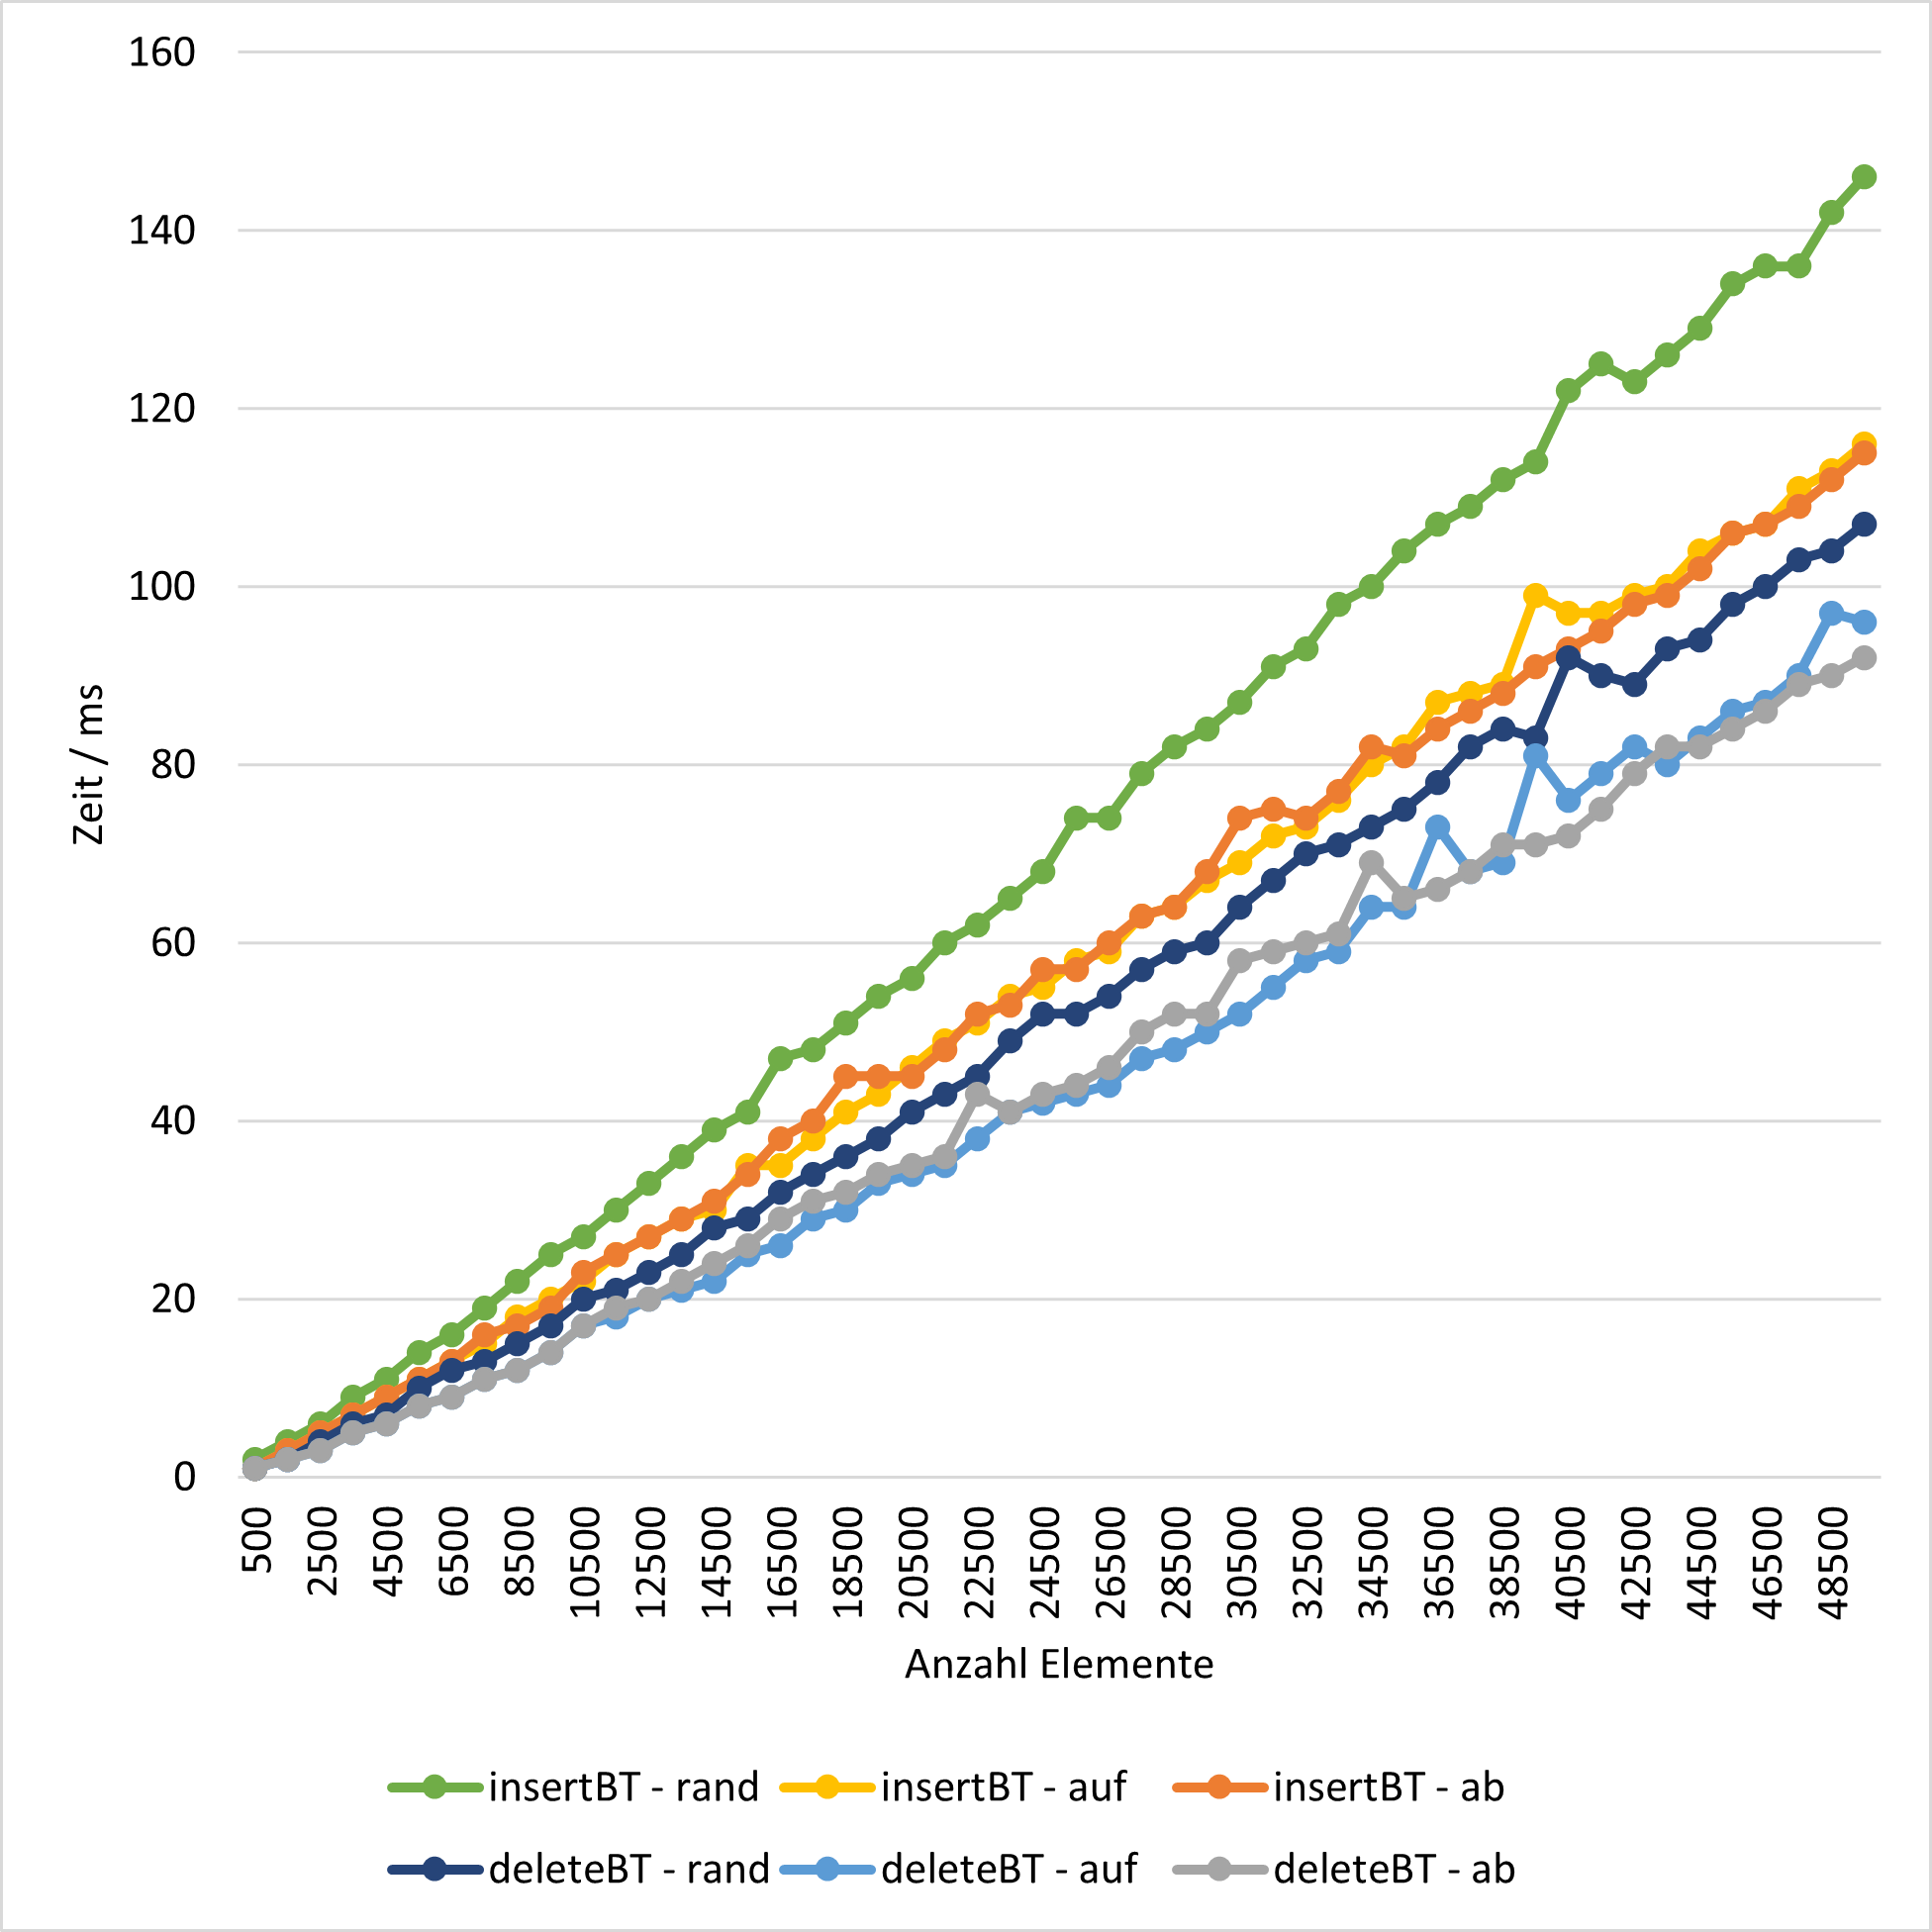
\includegraphics[width = 0.45\textwidth]
        {img/excel/avl1.png}\label{fig:avl-zeit-kummuliert}}
    \qquad
    \subfloat[\centering Pro Element - DeleteBT und InsertBT]{
        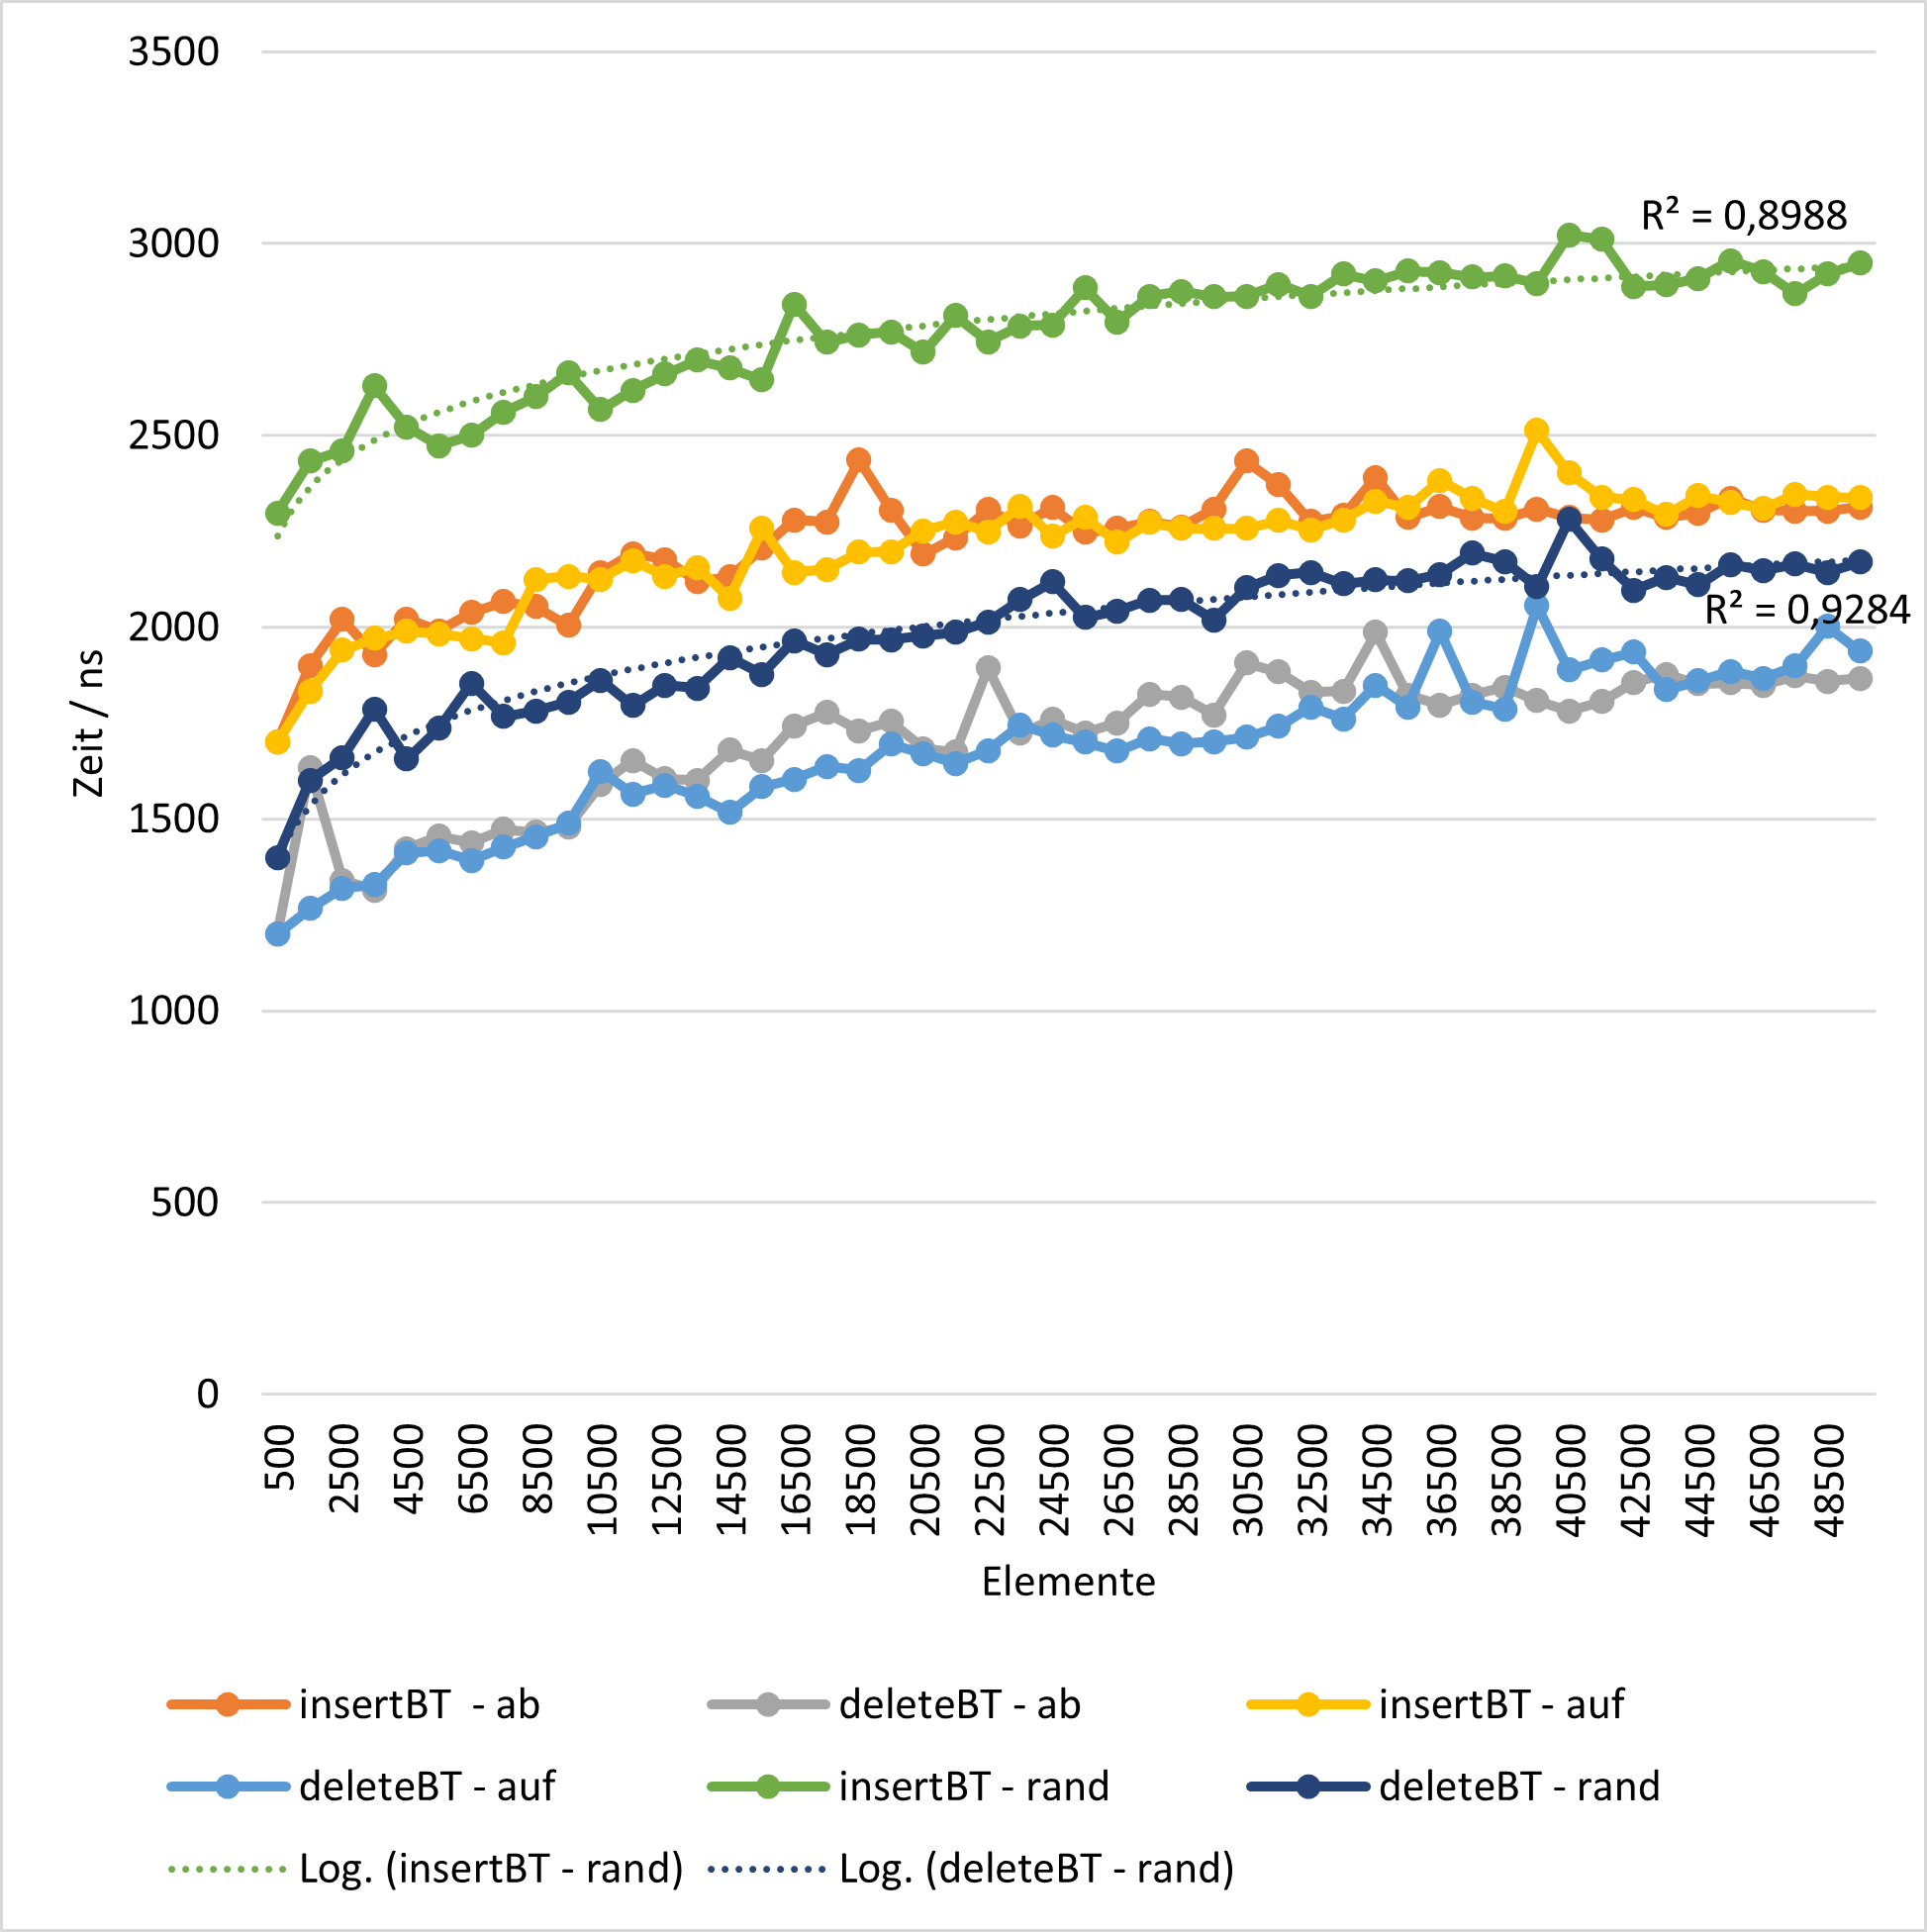
\includegraphics[width = 0.45\textwidth]
        {img/excel/avl1_el.png}\label{fig:avl-zeit-el-insert-delete}}
    \qquad
    \subfloat[\centering Pro Element - EqualBT und IsBT]{
        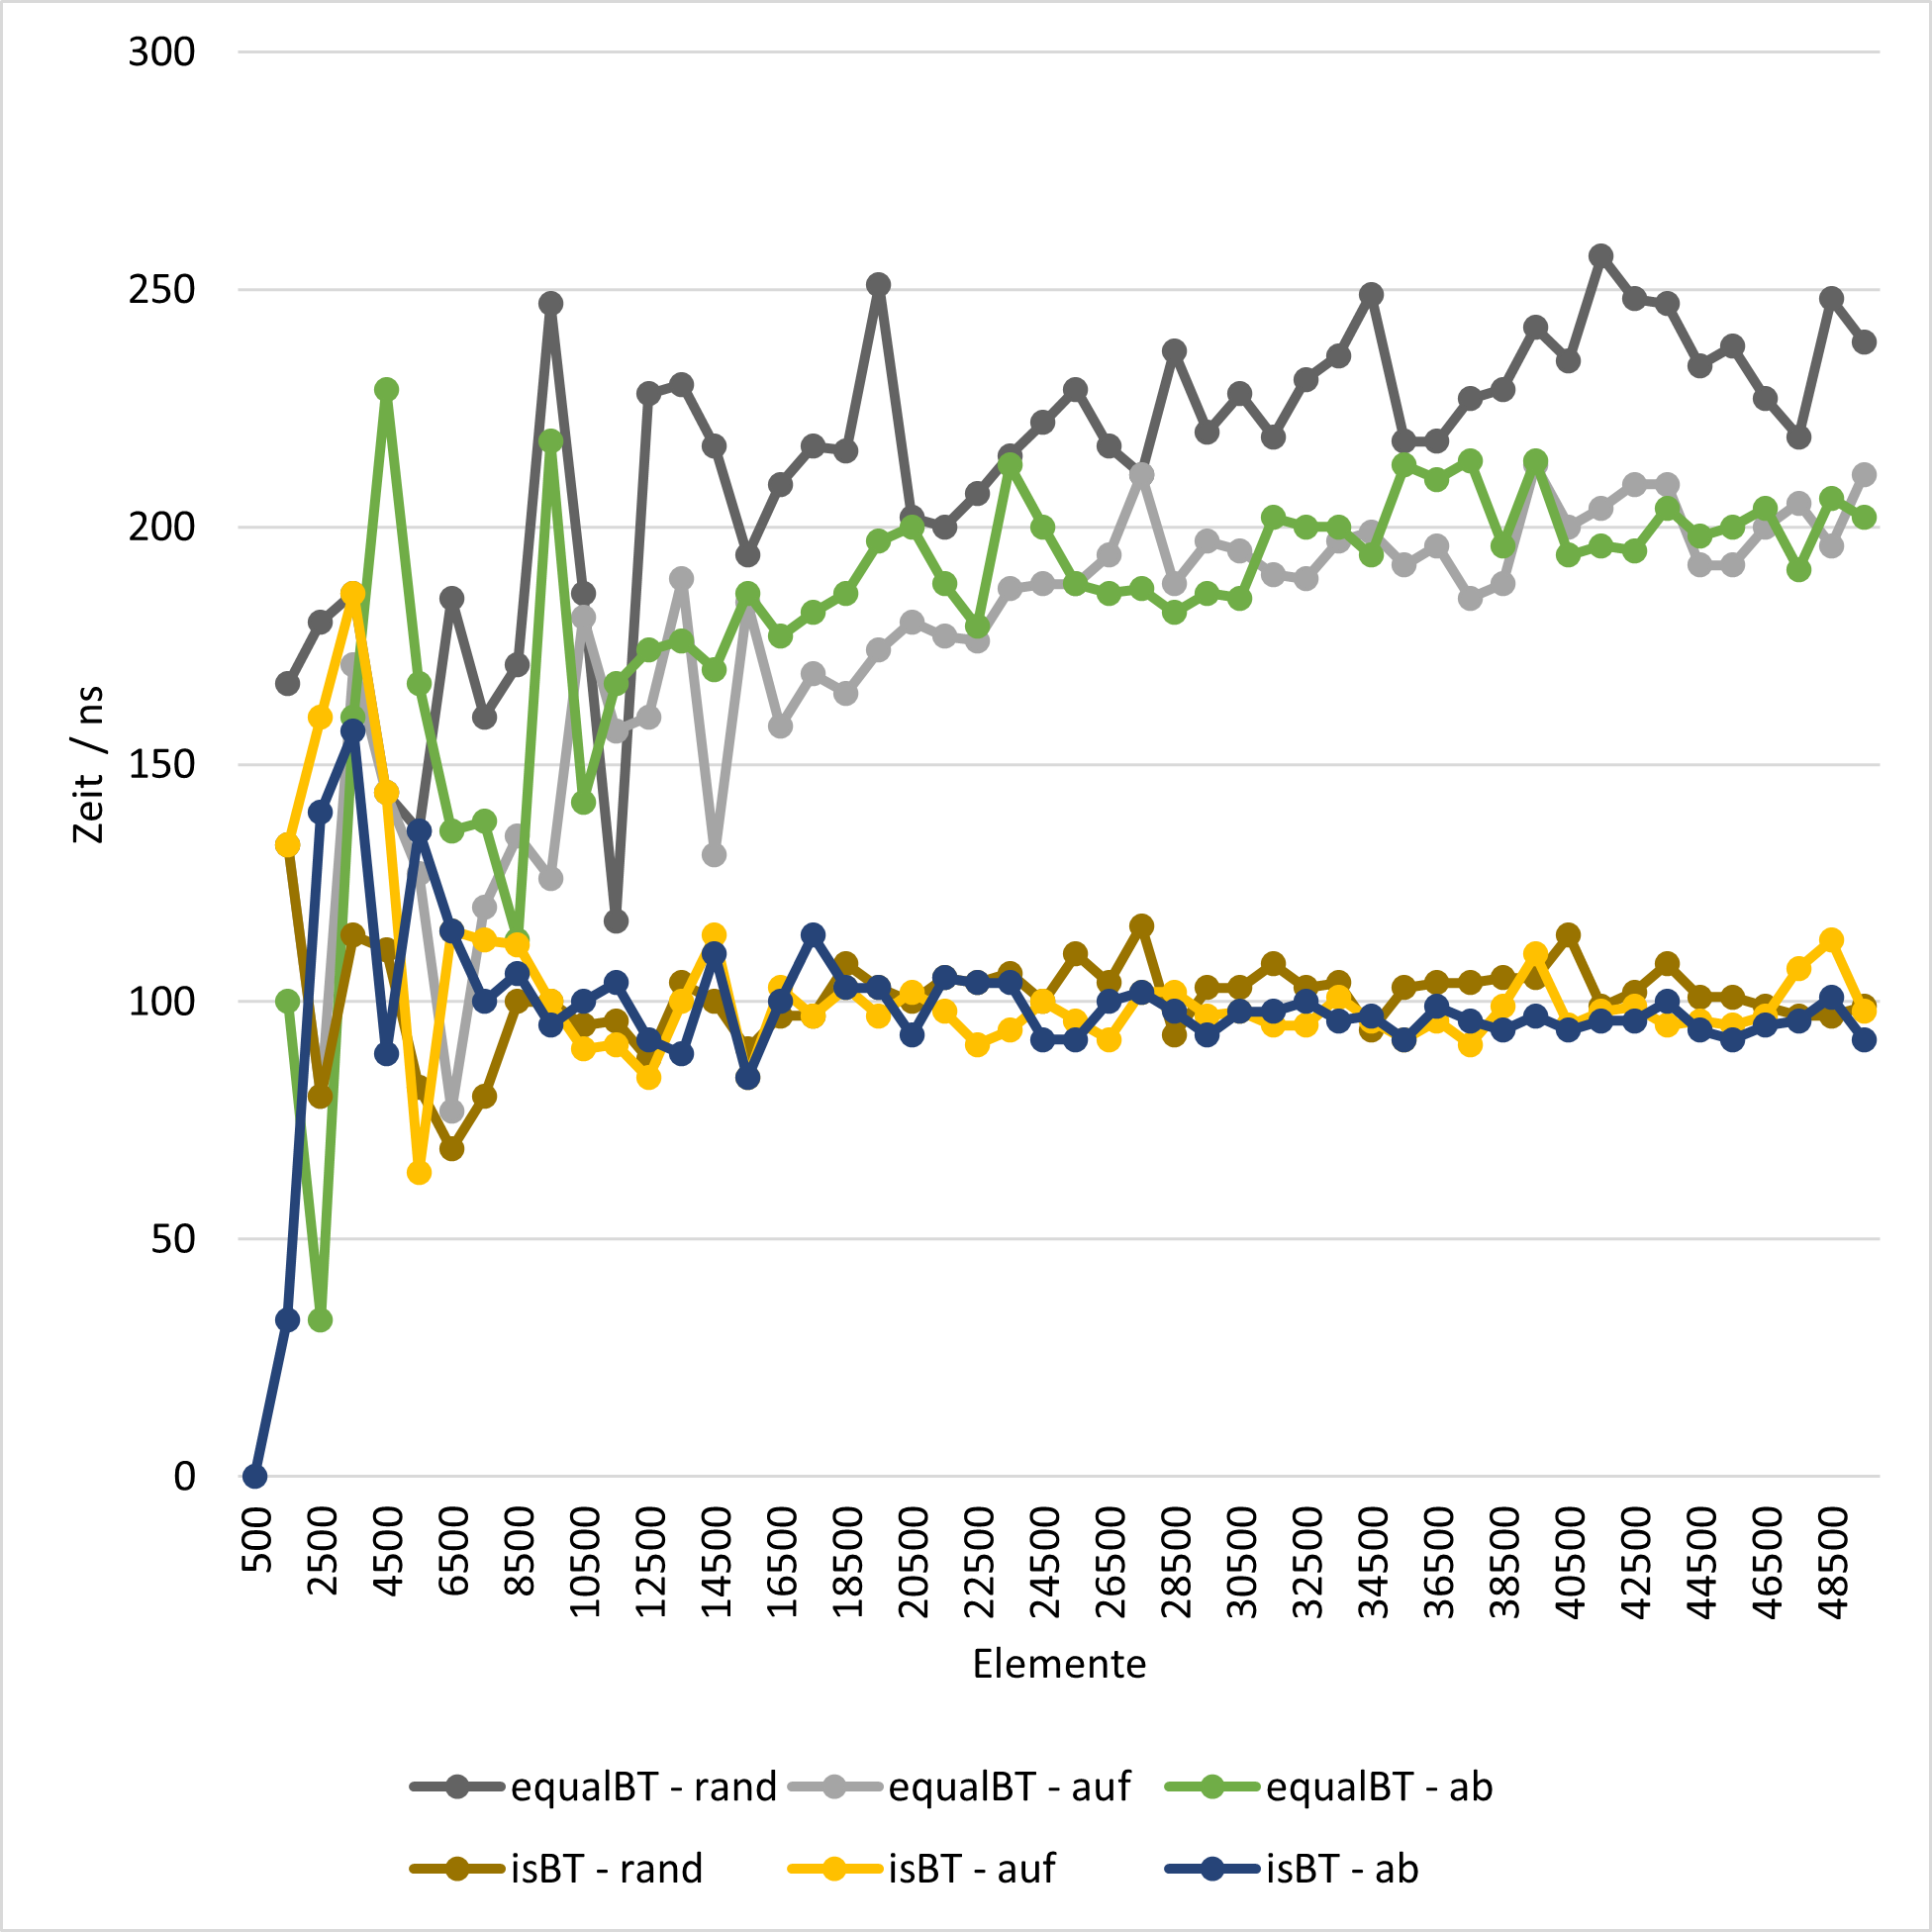
\includegraphics[width = 0.45\textwidth]
        {img/excel/avl2_el.png}\label{fig:avl-zeit-el-eq-is}}
    \qquad
    \subfloat[\centering Pro Element - FindBT]{
        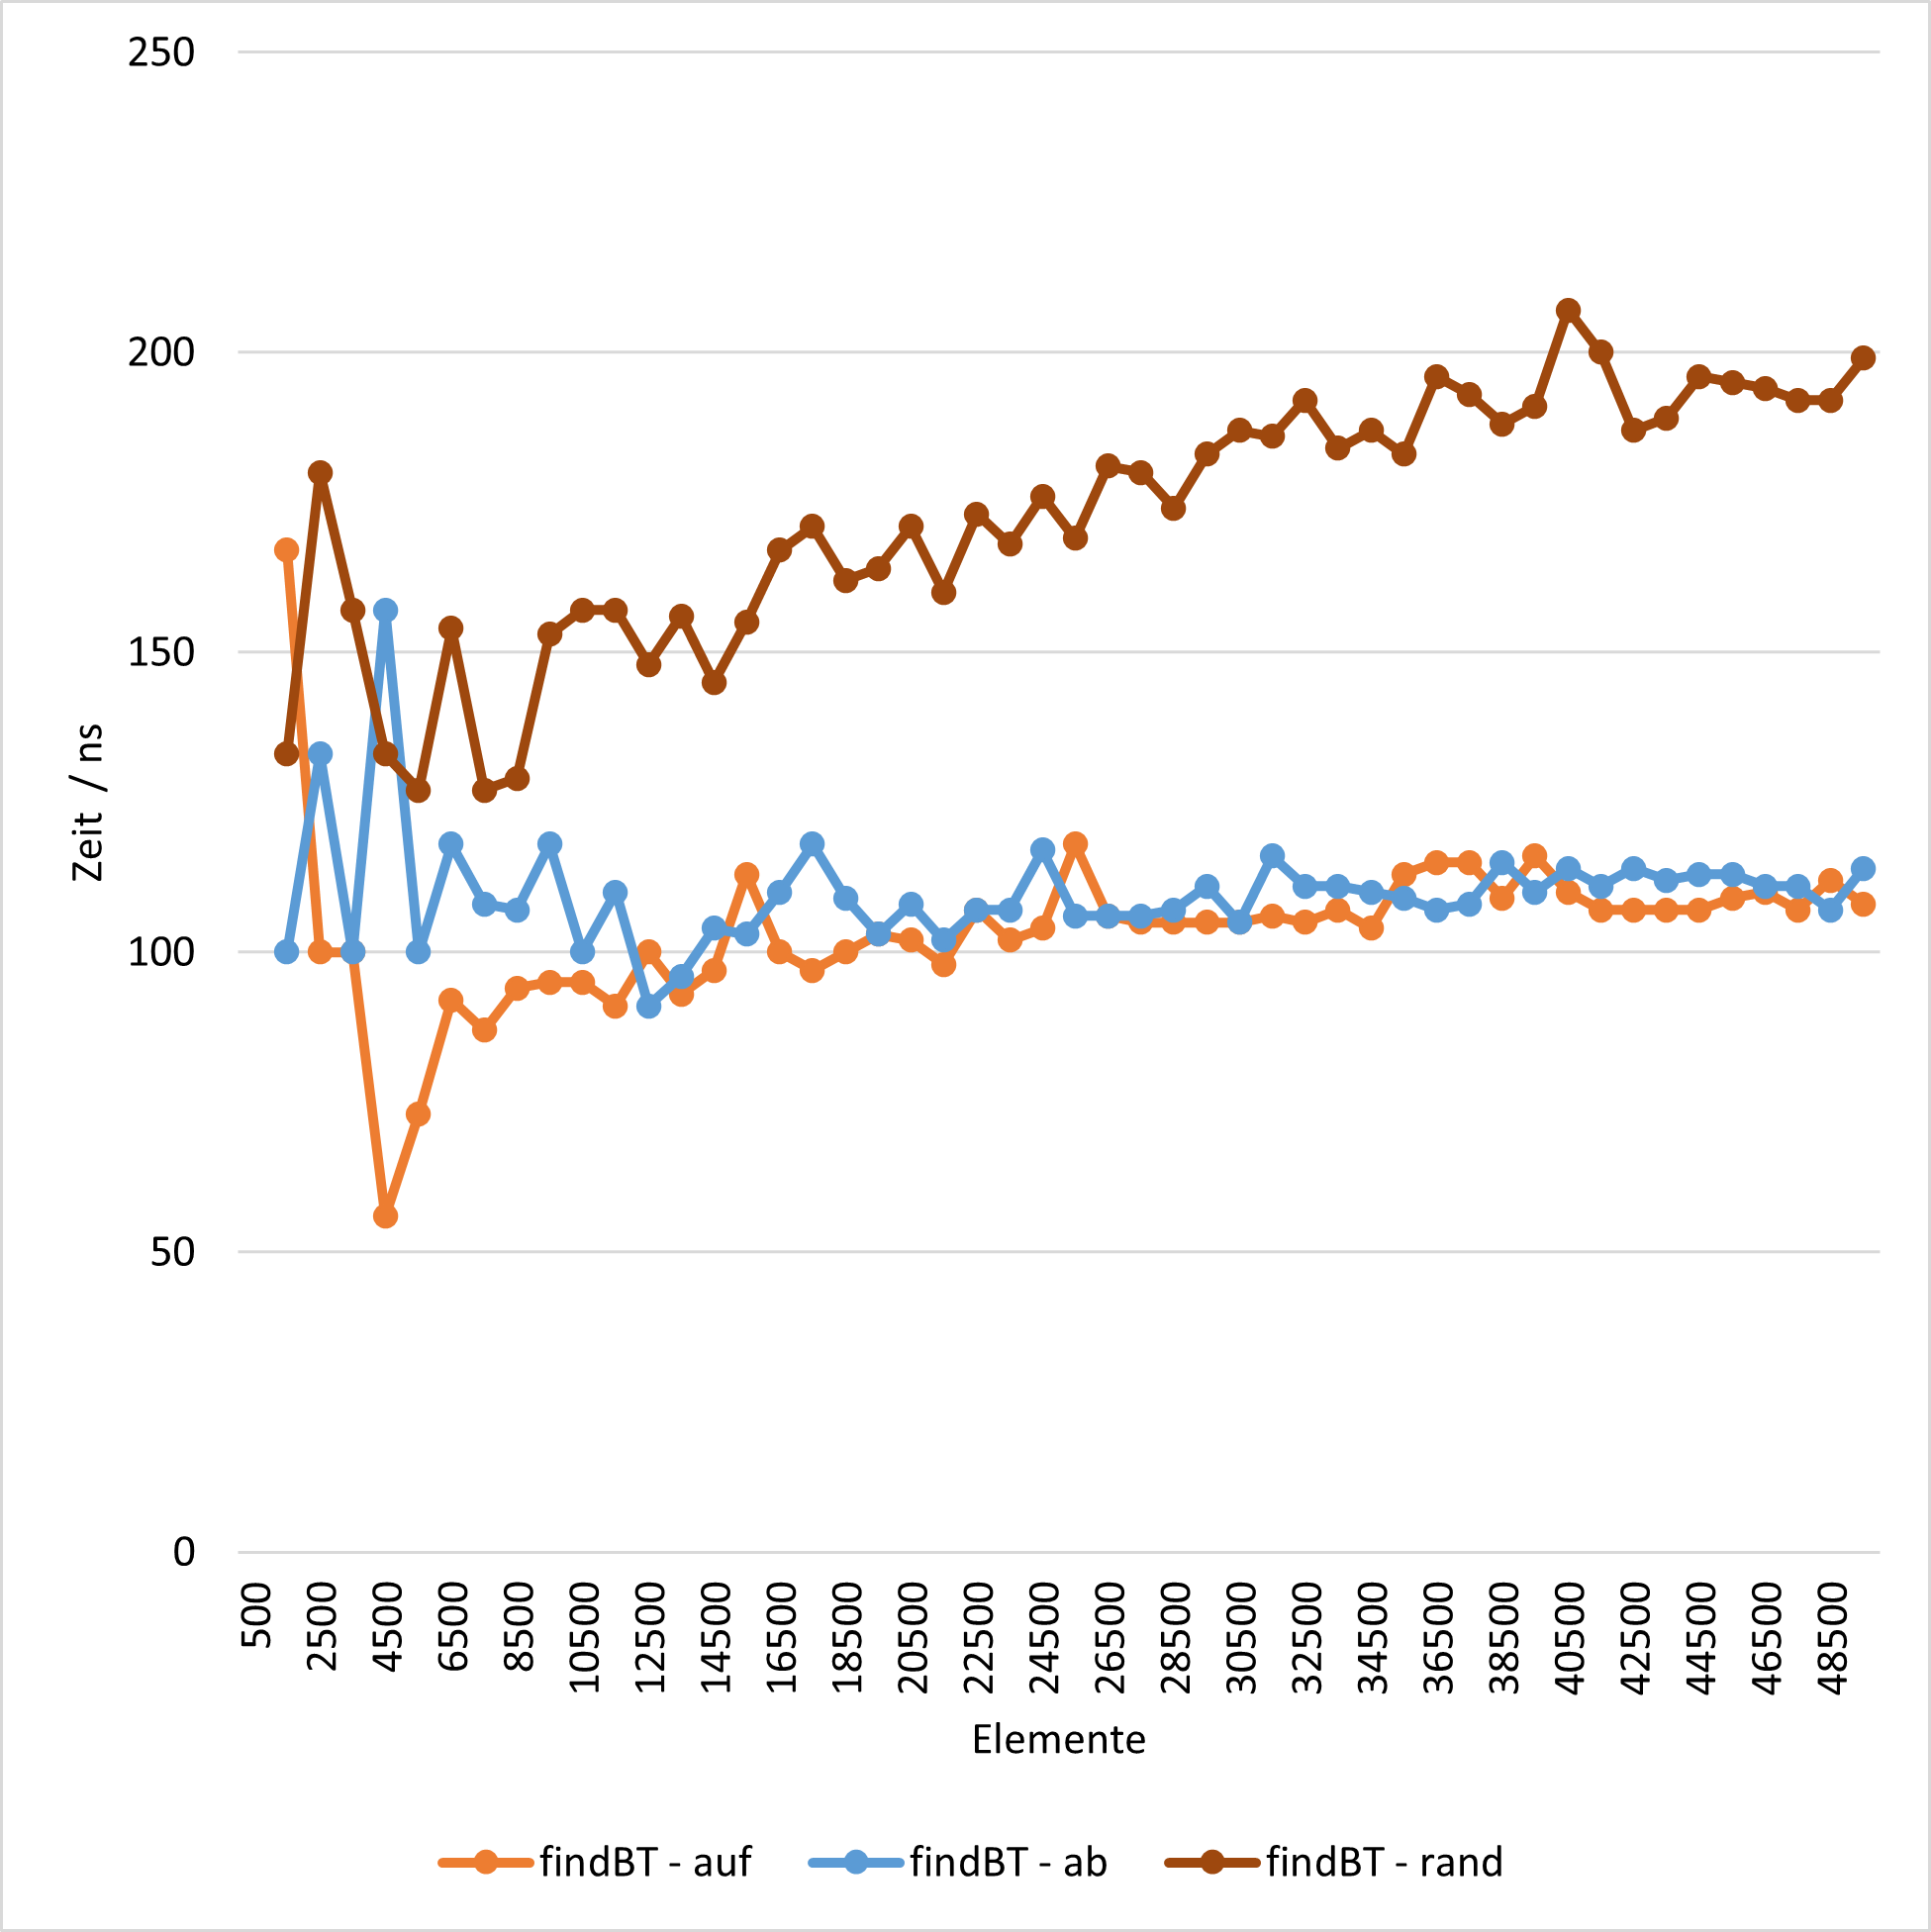
\includegraphics[width = 0.45\textwidth]
        {img/excel/avl3_el.png}\label{fig:avl-zeit-el-find}}
    \caption{Zeitmessungen AVL-Baum}
    \label{fig:avl_zeit}
\end{figure}

\subsection{Splay-Baum}
In Abbildung~\ref{fig:splay-zeit} und~\ref{fig:splay-zeit-rand} sind die Laufzeiten
kumuliert, in Abbildung~\ref{fig:splay-zeit-el} und~\ref{fig:splay-zeit-rand-el}
elementweise dargestellt.
Hier wurden, anders als bei der Zeitmessung vom AVL-Baum in
Abschnitt~\ref{subsec:laufzeitmessung-avl}, Balkendiagramme als Darstellungsart gewählt, da viele
Messwerte nahezu identisch sind und somit besser zu sehen sind.

Bei den Laufzeitemessungen ist zu beachten, dass die diese bei auf- und absteigenden
Zahlen nur bis zu 10500 Elementen durchgeführt wurden, da die Laufzeit dieser deutlich
länger als bei zufälligen ist.
Außerdem ist bei den kumulierten Messungen in~\ref{fig:splay-zeit} \textit{FindTP} und
in~\ref{fig:splay-zeit-rand} \textit{FindBT} auf der x-Achse abgeschnitten.

\paragraph{Auf- / Absteigende vs. zufällige Zahlen}
Bei auf- und absteigenden Zahlen fällt an Abbildung~\ref{fig:splay-zeit} auf, dass \textit{InsertBT}
eine sehr schnelle Laufzeit aufweist.
Diese ist konstant.
Das liegt daran, dass bei sortierten Zahlen das neue Element jeweils an
der Wurzel angefügt wird, und anschließend einmal rotiert wird, sodass dieses Element die
neue Wurzel darstellt.
Somit ist der Aufwand bei jedem Einfügen gleich hoch.

Des Weiteren ist die Laufzeit von \textit{EqualBT} bei aufsteigenden Zahlen sehr schnell,
wobei diese bei absteigenden Zahlen deutlich langsamer ist.
Dies lässt sich durch die Implementation der \textit{EqualBT}-Methode erklären:
Der Baum wird zunächst in aufsteigend sortierter Reihenfolge als Liste ausgegeben,
anschließend wird diese Liste auf Gleichheit überprüft.
Da beim Einfügen von sortieren Elementen diese an der Wurzel eingefügt werden, wird die
Reihenfolge des Baumes umgekehrt.
Somit ist ein Baum nach dem Einfügen von aufsteigend sortierten Elementen absteigend sortiert
und muss von der \textit{EqualBT}-Methode umgekehrt werden.
Dies ist in Erlang besonders aufwendig, da beim Anfügen an eine Liste jedes Mal bis ans Ende
der Liste gelaufen werden muss.
Der Baum, in den die Elemente absteigend sortiert eingefügt wurden, ist hingegen bereits
aufsteigend sortiert.
Der Aufwand für das Umkehren der Liste entfällt somit.
In Abbildung~\ref{fig:splay-zeit-rand-el} ist zu erkennen, dass die
Laufzeit von \textit{EqualBT} bei zufälligen Zahlen niedriger ist,
als bei aufsteigenden, jedoch höher als bei absteigendenden Zahlen.
So beträgt die Laufzeit bei 10500 Elementen bei zufälligen Zahlen beispielsweise ca. 250ms,
bei aufsteigenden Zahlen ca. 1100ms.


\paragraph{FindBT vs. FindTP}
In Abbildung~\ref{fig:splay-bt-vs-tp} ist \textit{FindTP} auch bei auf- und absteigenden Zahlen
dargestellt.
Der Graph von \textit{FindTP} scheint bis zu ca 5500 Elementen quadratisch zu verlaufen, danach
führt dieser linear fort.
Es wird deutlich, dass im Fall von sortieren Zahlen nicht häufig genug rotiert, um
die zugegriffenen Elemente nach oben zu rotieren.
Somit ist die Komplexität von \textit{FindTP} in diesem Fall nicht mehr logarithmisch.
Falls auf ein Element, welches sich weit unten im Baum befindet, häufig zugegriffen wird, wird
dieses jeweils nur eine Position gesplayt, dies ist bei einem großem Baum sehr aufwendig.

Im Falle von zufälligen Zahlen (Abbildung~\ref{fig:splay-zeit-rand-el}) erweist sich \textit{FindTP}
als das schnellere der beiden Verfahren.
\textit{FindBT} ist bis zu 8 Mal langsamer, was sich dadurch erklären lässt, dass der Overhead
der Rotationen zu hoch ist.
Dadurch, dass die Elemente zufällig eingefügt wurden, ist der Baum am Anfang einigermaßen
ausgeglichen.
Die Zugriffszeit auf ein Element ist somit nicht hoch genug, dass es sich lohnen würde,
dieses Element komplett nach oben zu rotieren.
Dabei ist zu bedenken, dass, durch die Funktionsweise von Erlang, Rotationen sehr teuer sind, da
die Knoten jedes Mal neu erstellt werden müssen, also Speicherplatz alloziert wird.
In einer Sprache, in der mit veränderlichen Variablen gearbeitet wird, könnte \textit{FindBT}
eine bessere Laufzeit aufweisen.

Zusammenfassen lässt sich sagen, dass \textit{FindBT} eine konstantere Laufzeit bei
unterschiedlichen Bedingungen aufweist, wobei \textit{FindTP} bei zufälligen Zahlen
schneller, jedoch bei sortierten Zahlen deutlich langsamer ist.
Da die Komplexität von dem letzteren Verfahren bei sortierten Zahlen nicht mehr
logarithmisch ist, ist \textit{FindBT} vorzuziehen, wenn sortierte Zahlen nicht ausgeschlossen sind.


\paragraph{Komplexität}
In Abbildung~\ref{fig:splay-zeit-el} und~\ref{fig:splay-zeit-rand-el} sind jeweils
logarithmische Regressionen für \textit{DeleteBT}, \textit{FindBT} und \textit{FindTP} eingezeichnet.
Alle Methoden zeigen ein logarithmisches Verhalten.
Lediglich \textit{FindTP} scheint bei zufälligen Zahlen besser als logarithmisch zu sein.
\textit{FindTP} ist bei sortierten Zahlen (Abbildung~\ref{fig:splay-bt-vs-tp}), wie oben
beschrieben, nicht mehr logarithmisch.

\begin{figure}[hbt]
    \centering
    \subfloat[\centering Kumuliert - Auf- / Absteigend]{
        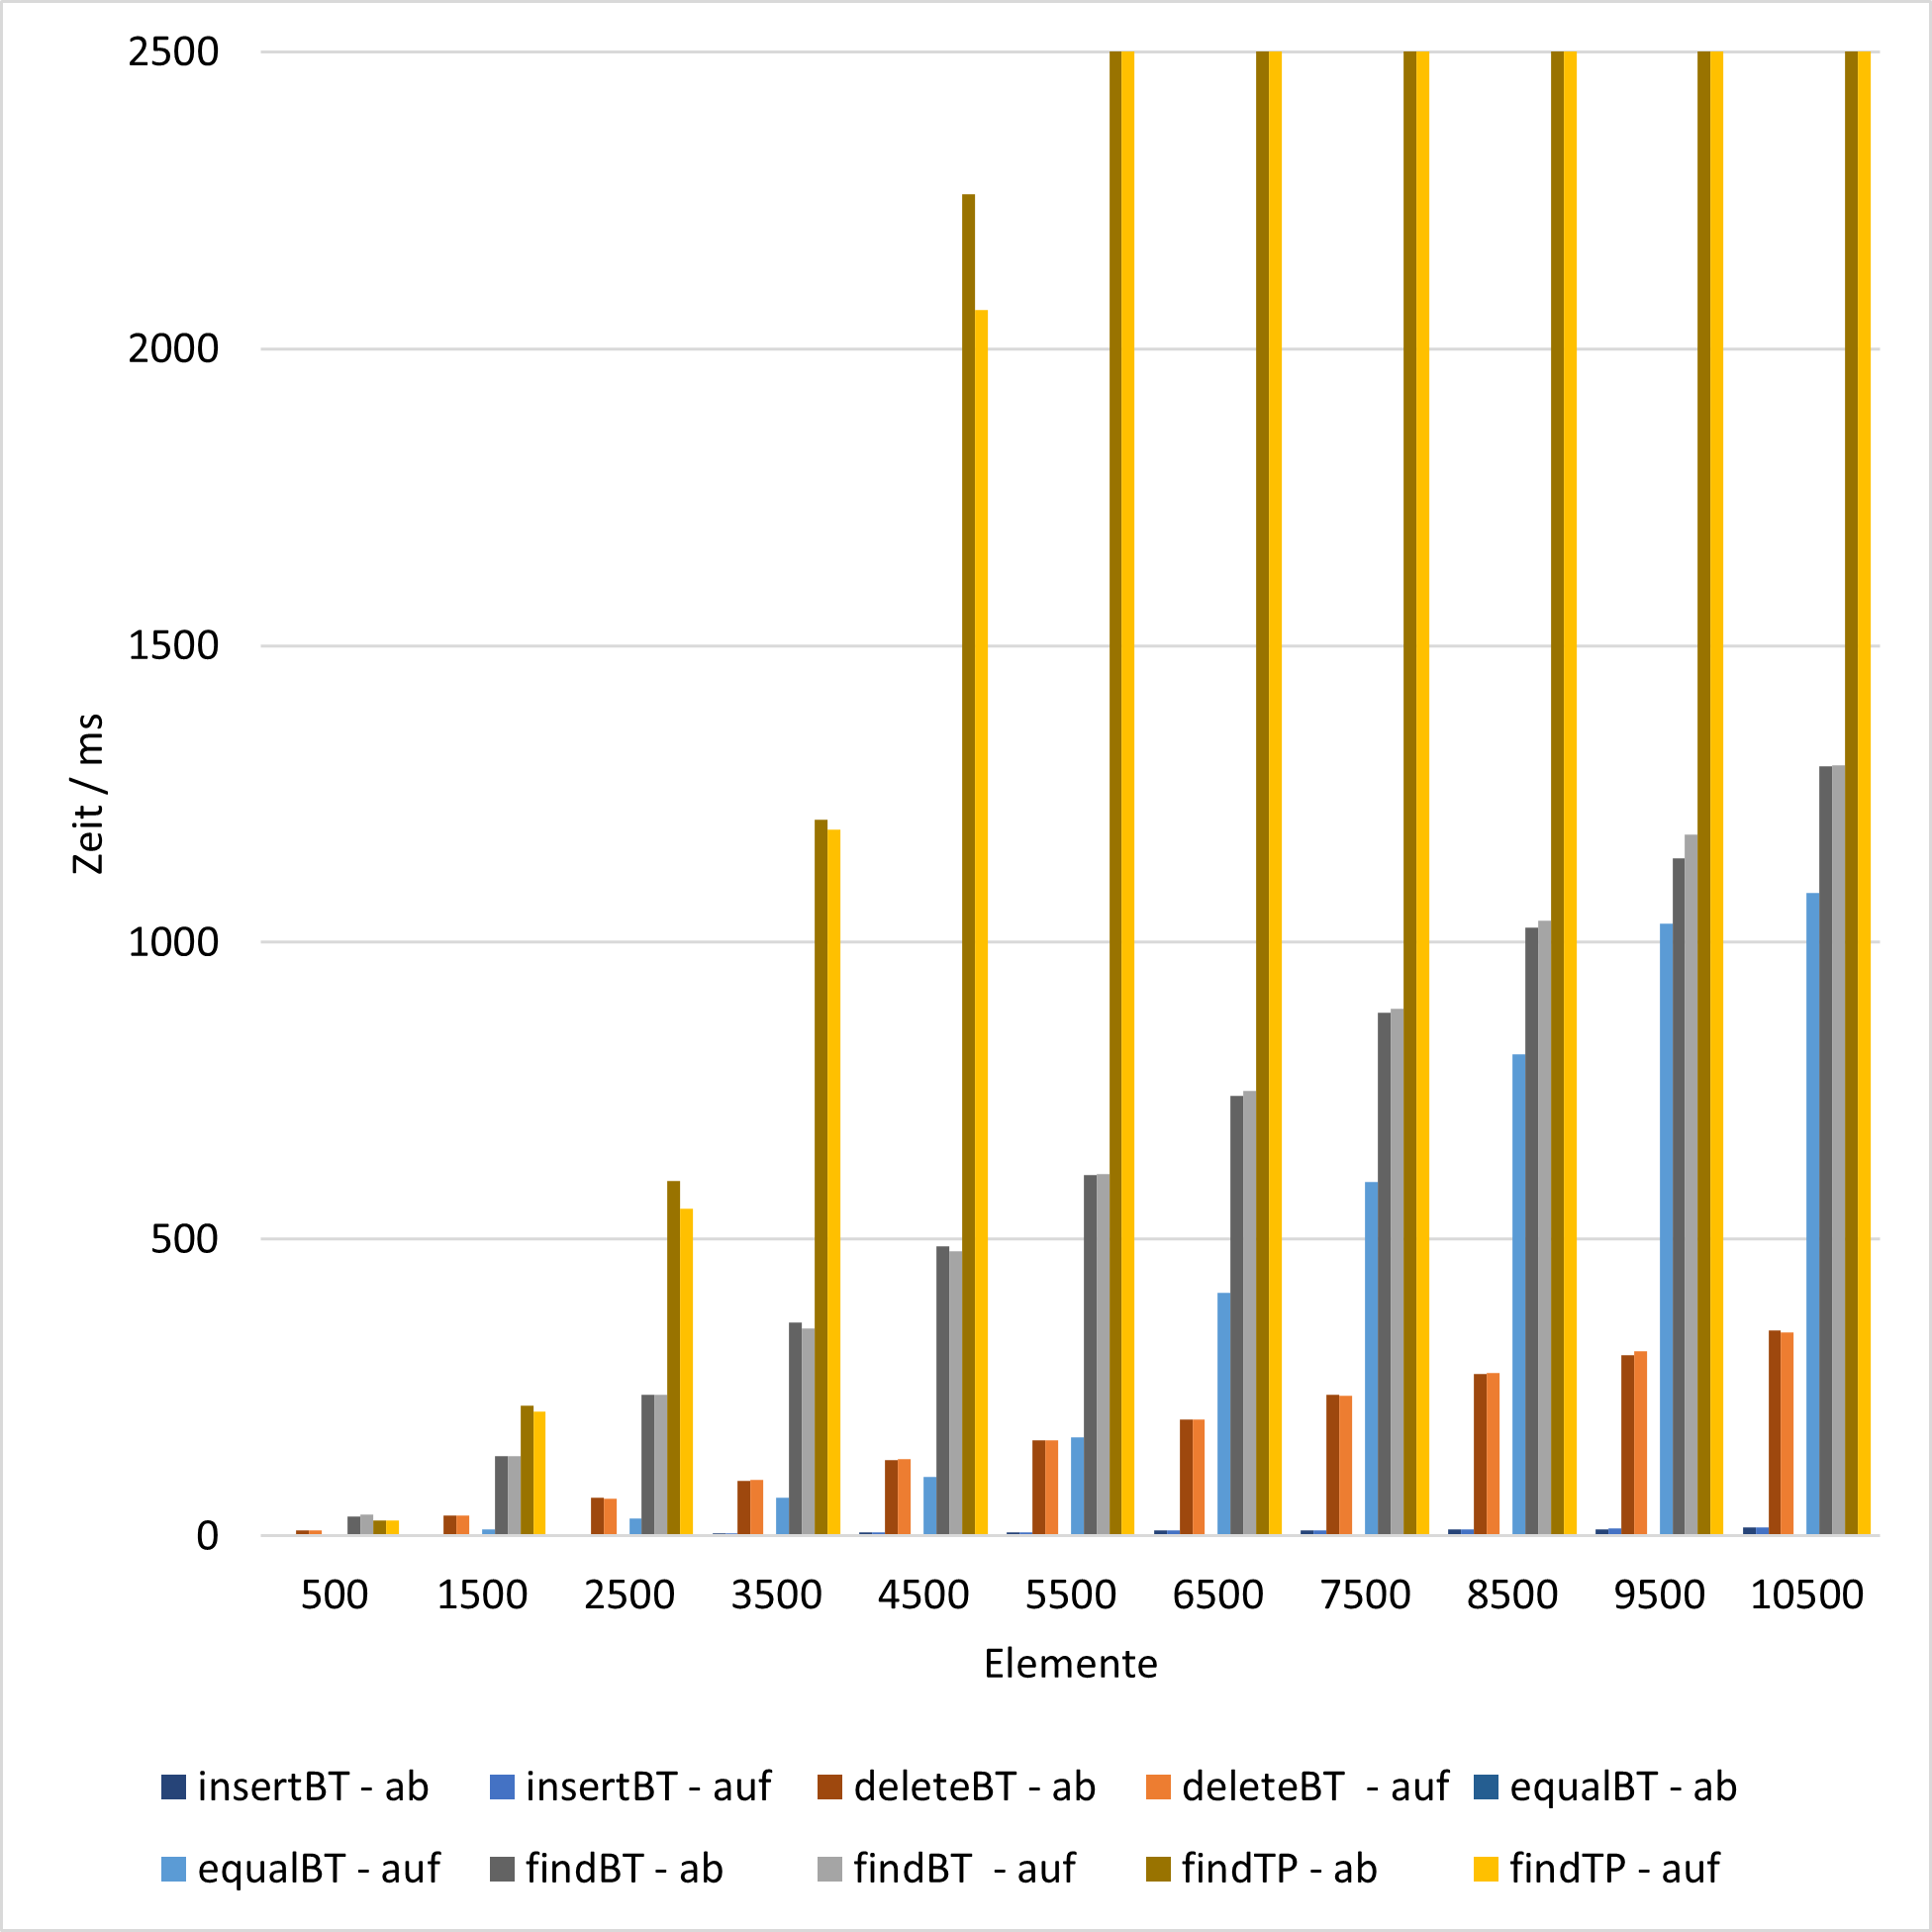
\includegraphics[width = 0.45\textwidth]
        {img/excel/splay1.png}\label{fig:splay-zeit}}
    \qquad
    \subfloat[\centering Kumuliert - Zufällig]{
        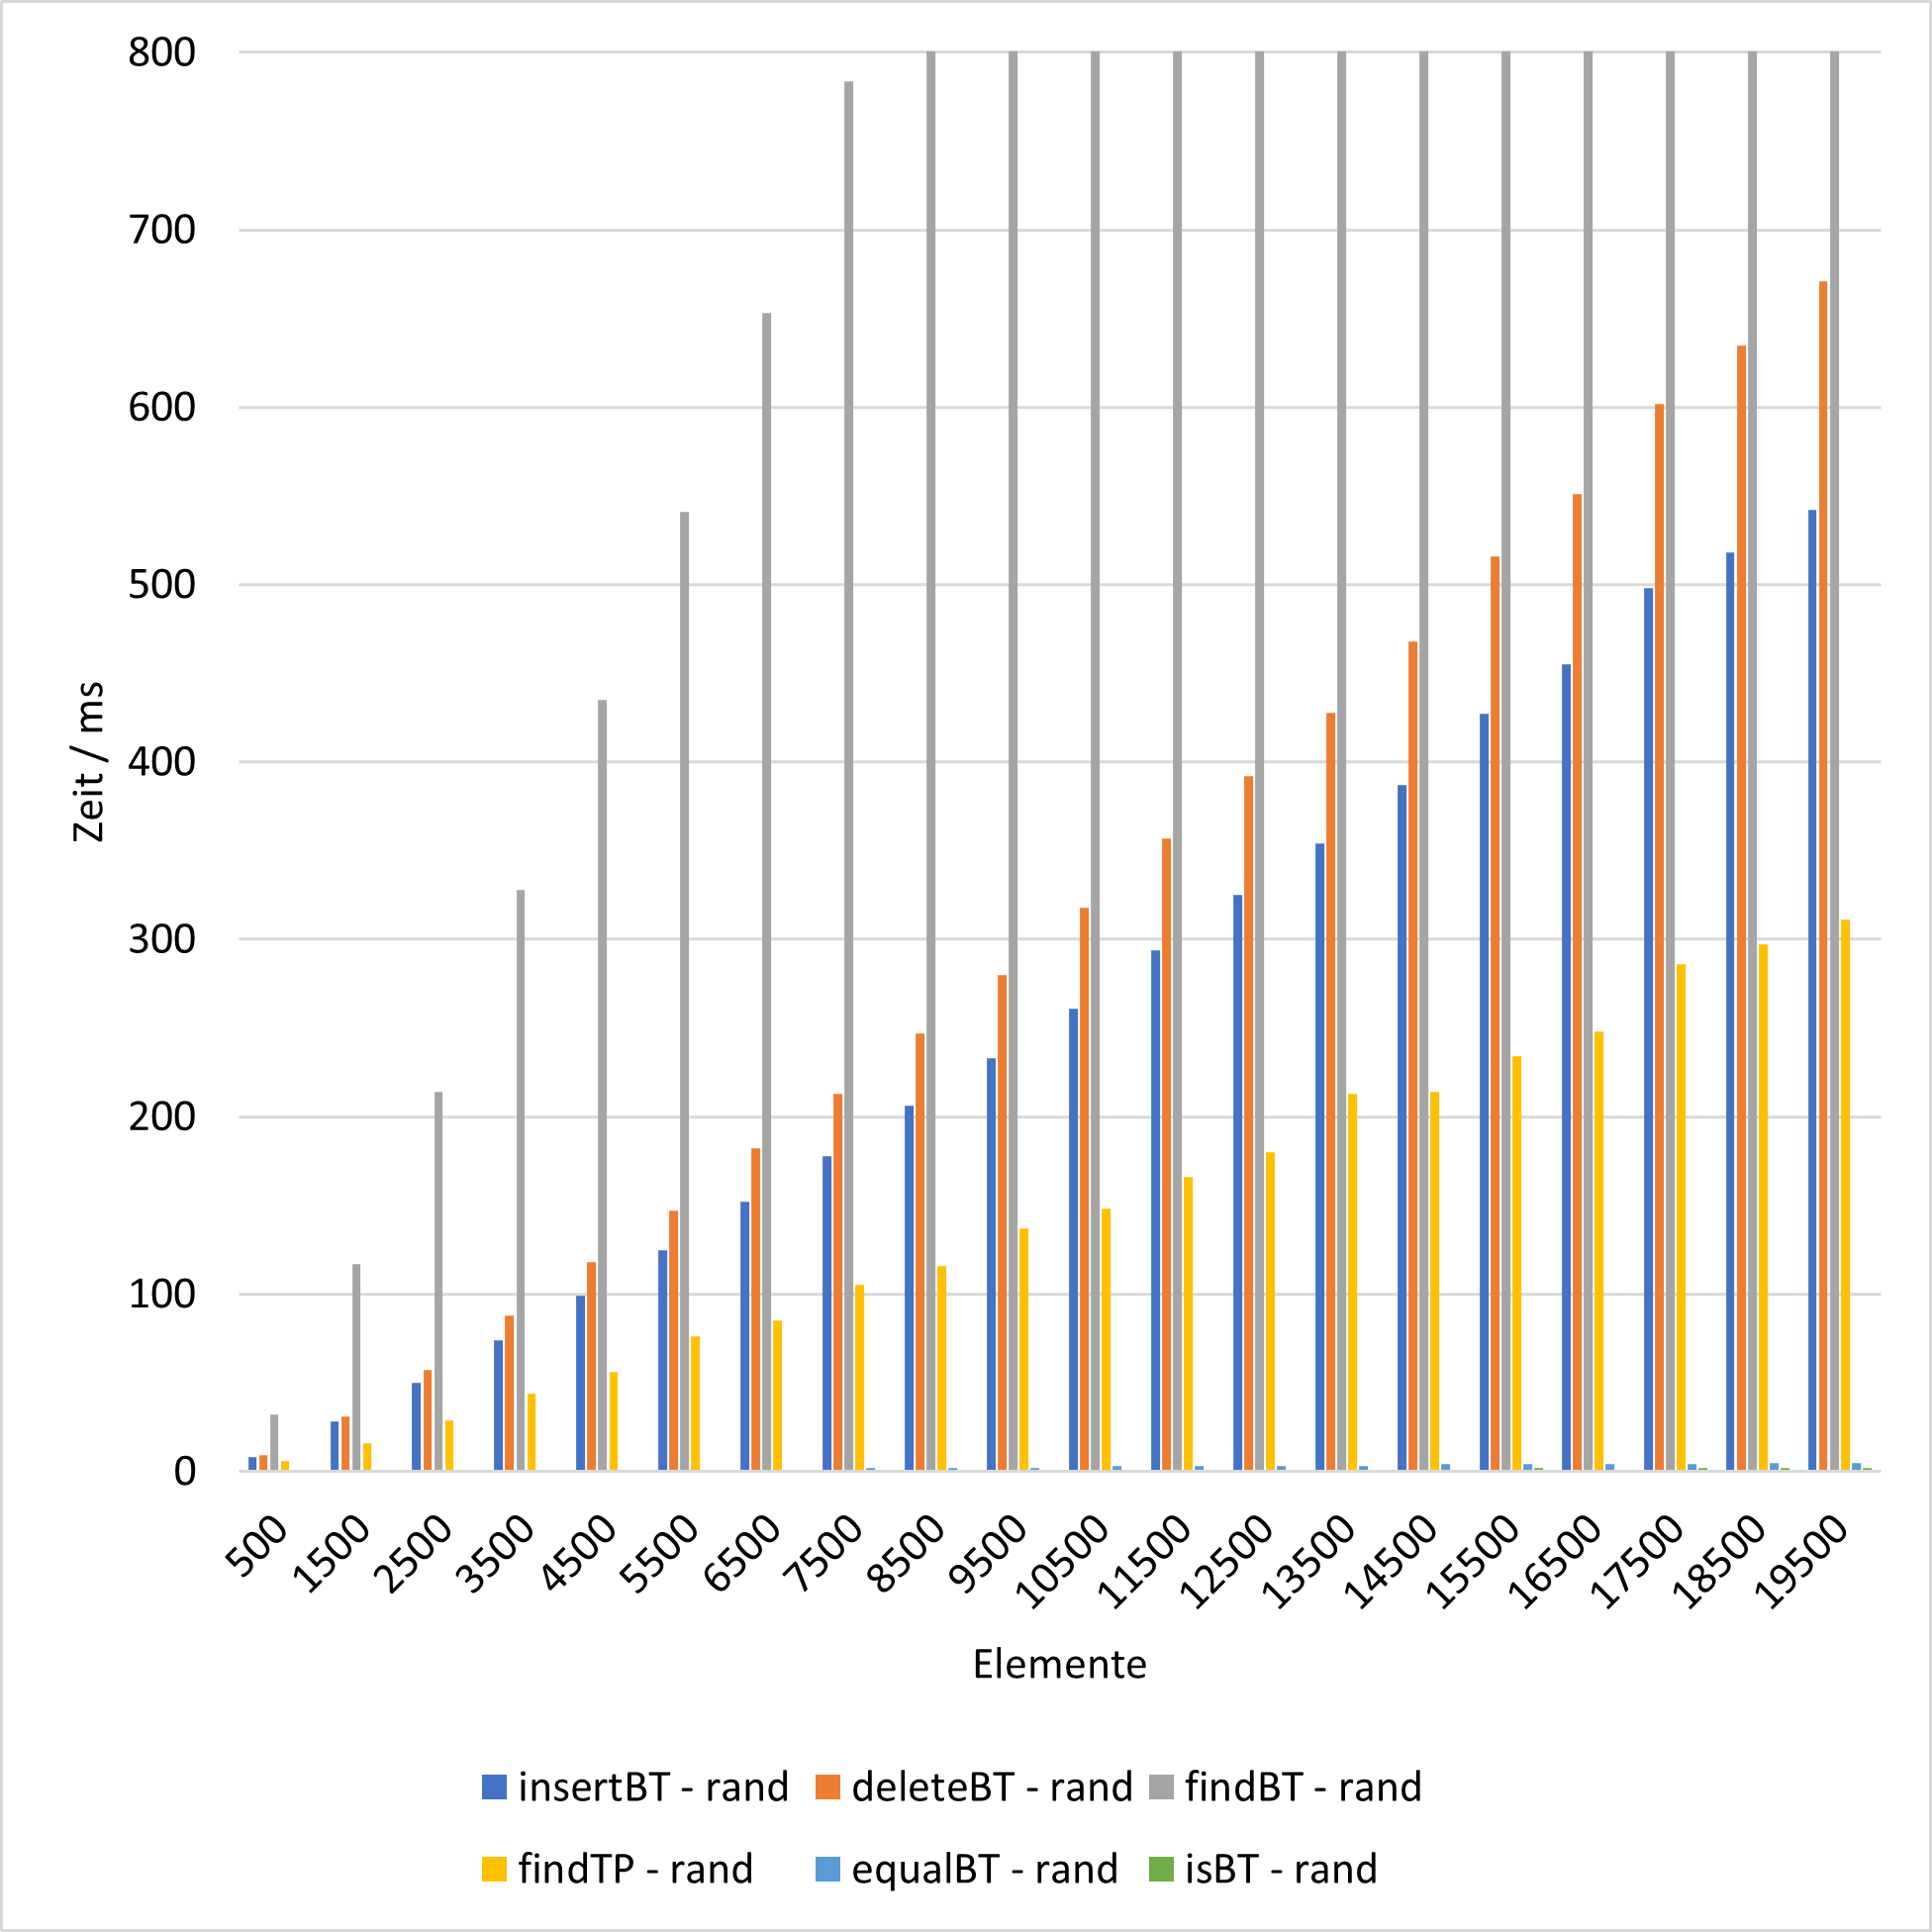
\includegraphics[width = 0.45\textwidth]
        {img/excel/splay_rand.png}\label{fig:splay-zeit-rand}}
    \qquad
    \subfloat[\centering Pro Element - Auf- / Absteigend]{
        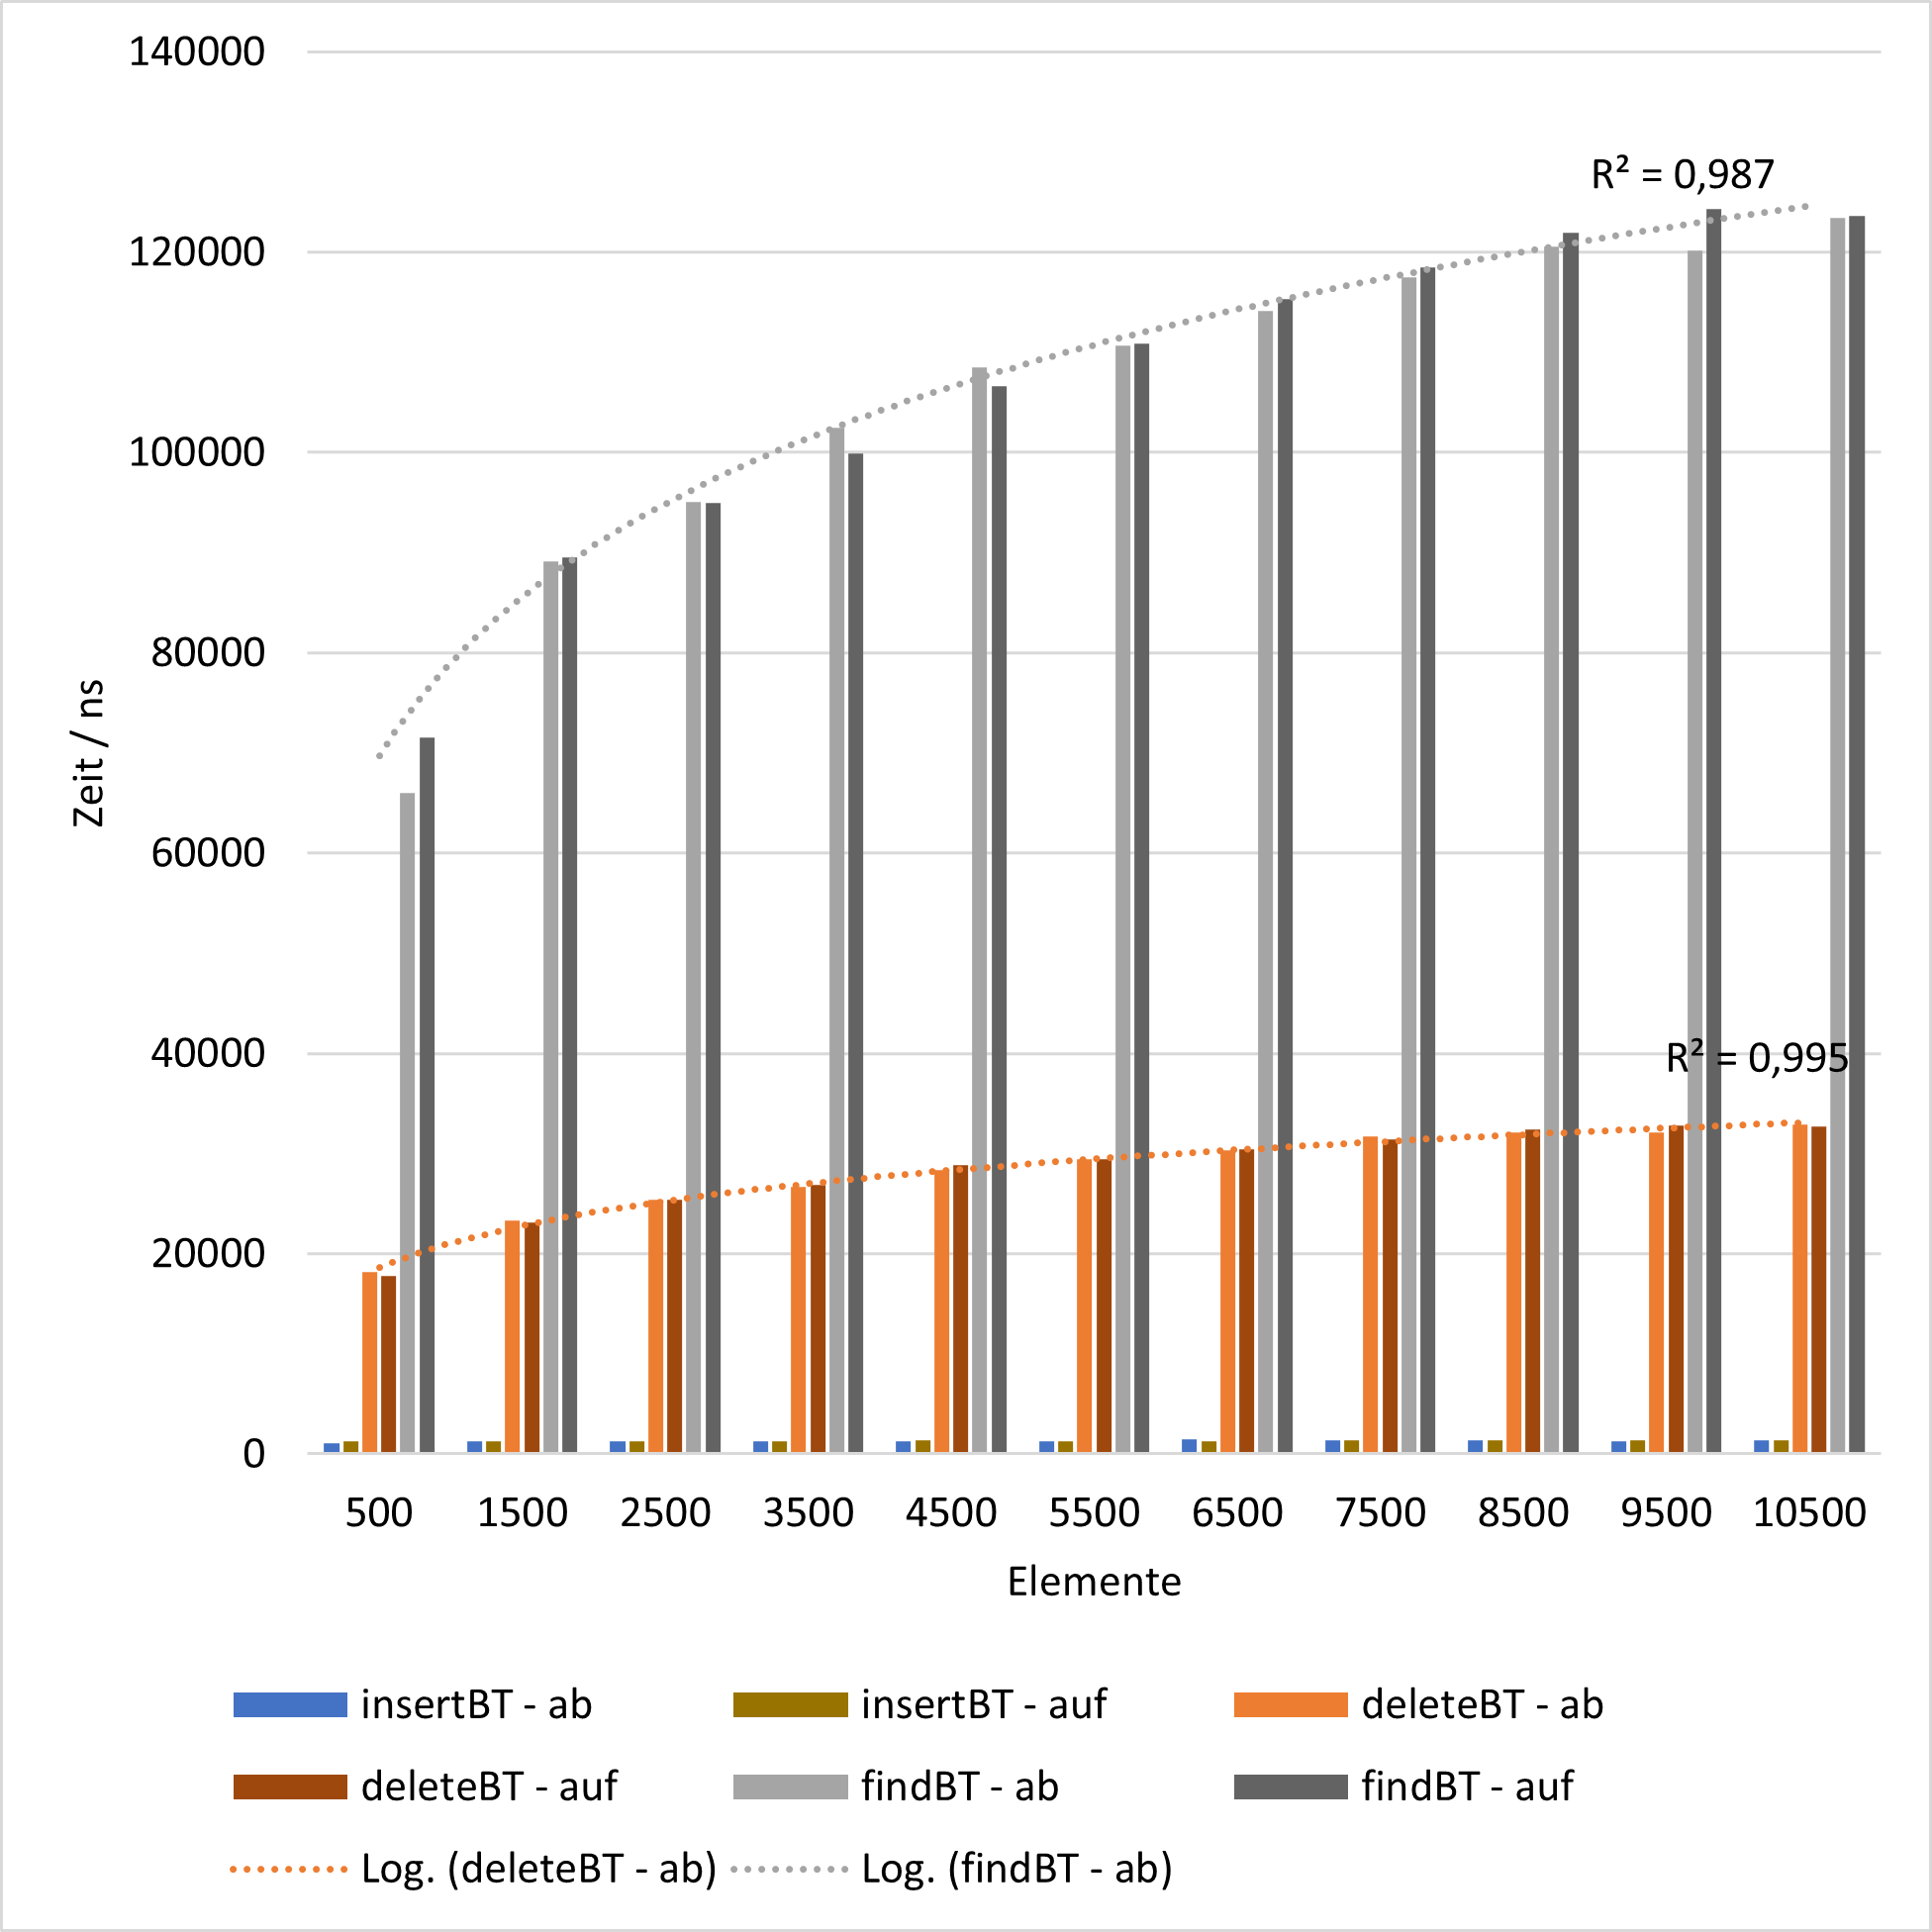
\includegraphics[width = 0.45\textwidth]
        {img/excel/splay1_el.png}\label{fig:splay-zeit-el}}
    \qquad
    \subfloat[\centering Pro Element - Zufällig]{
        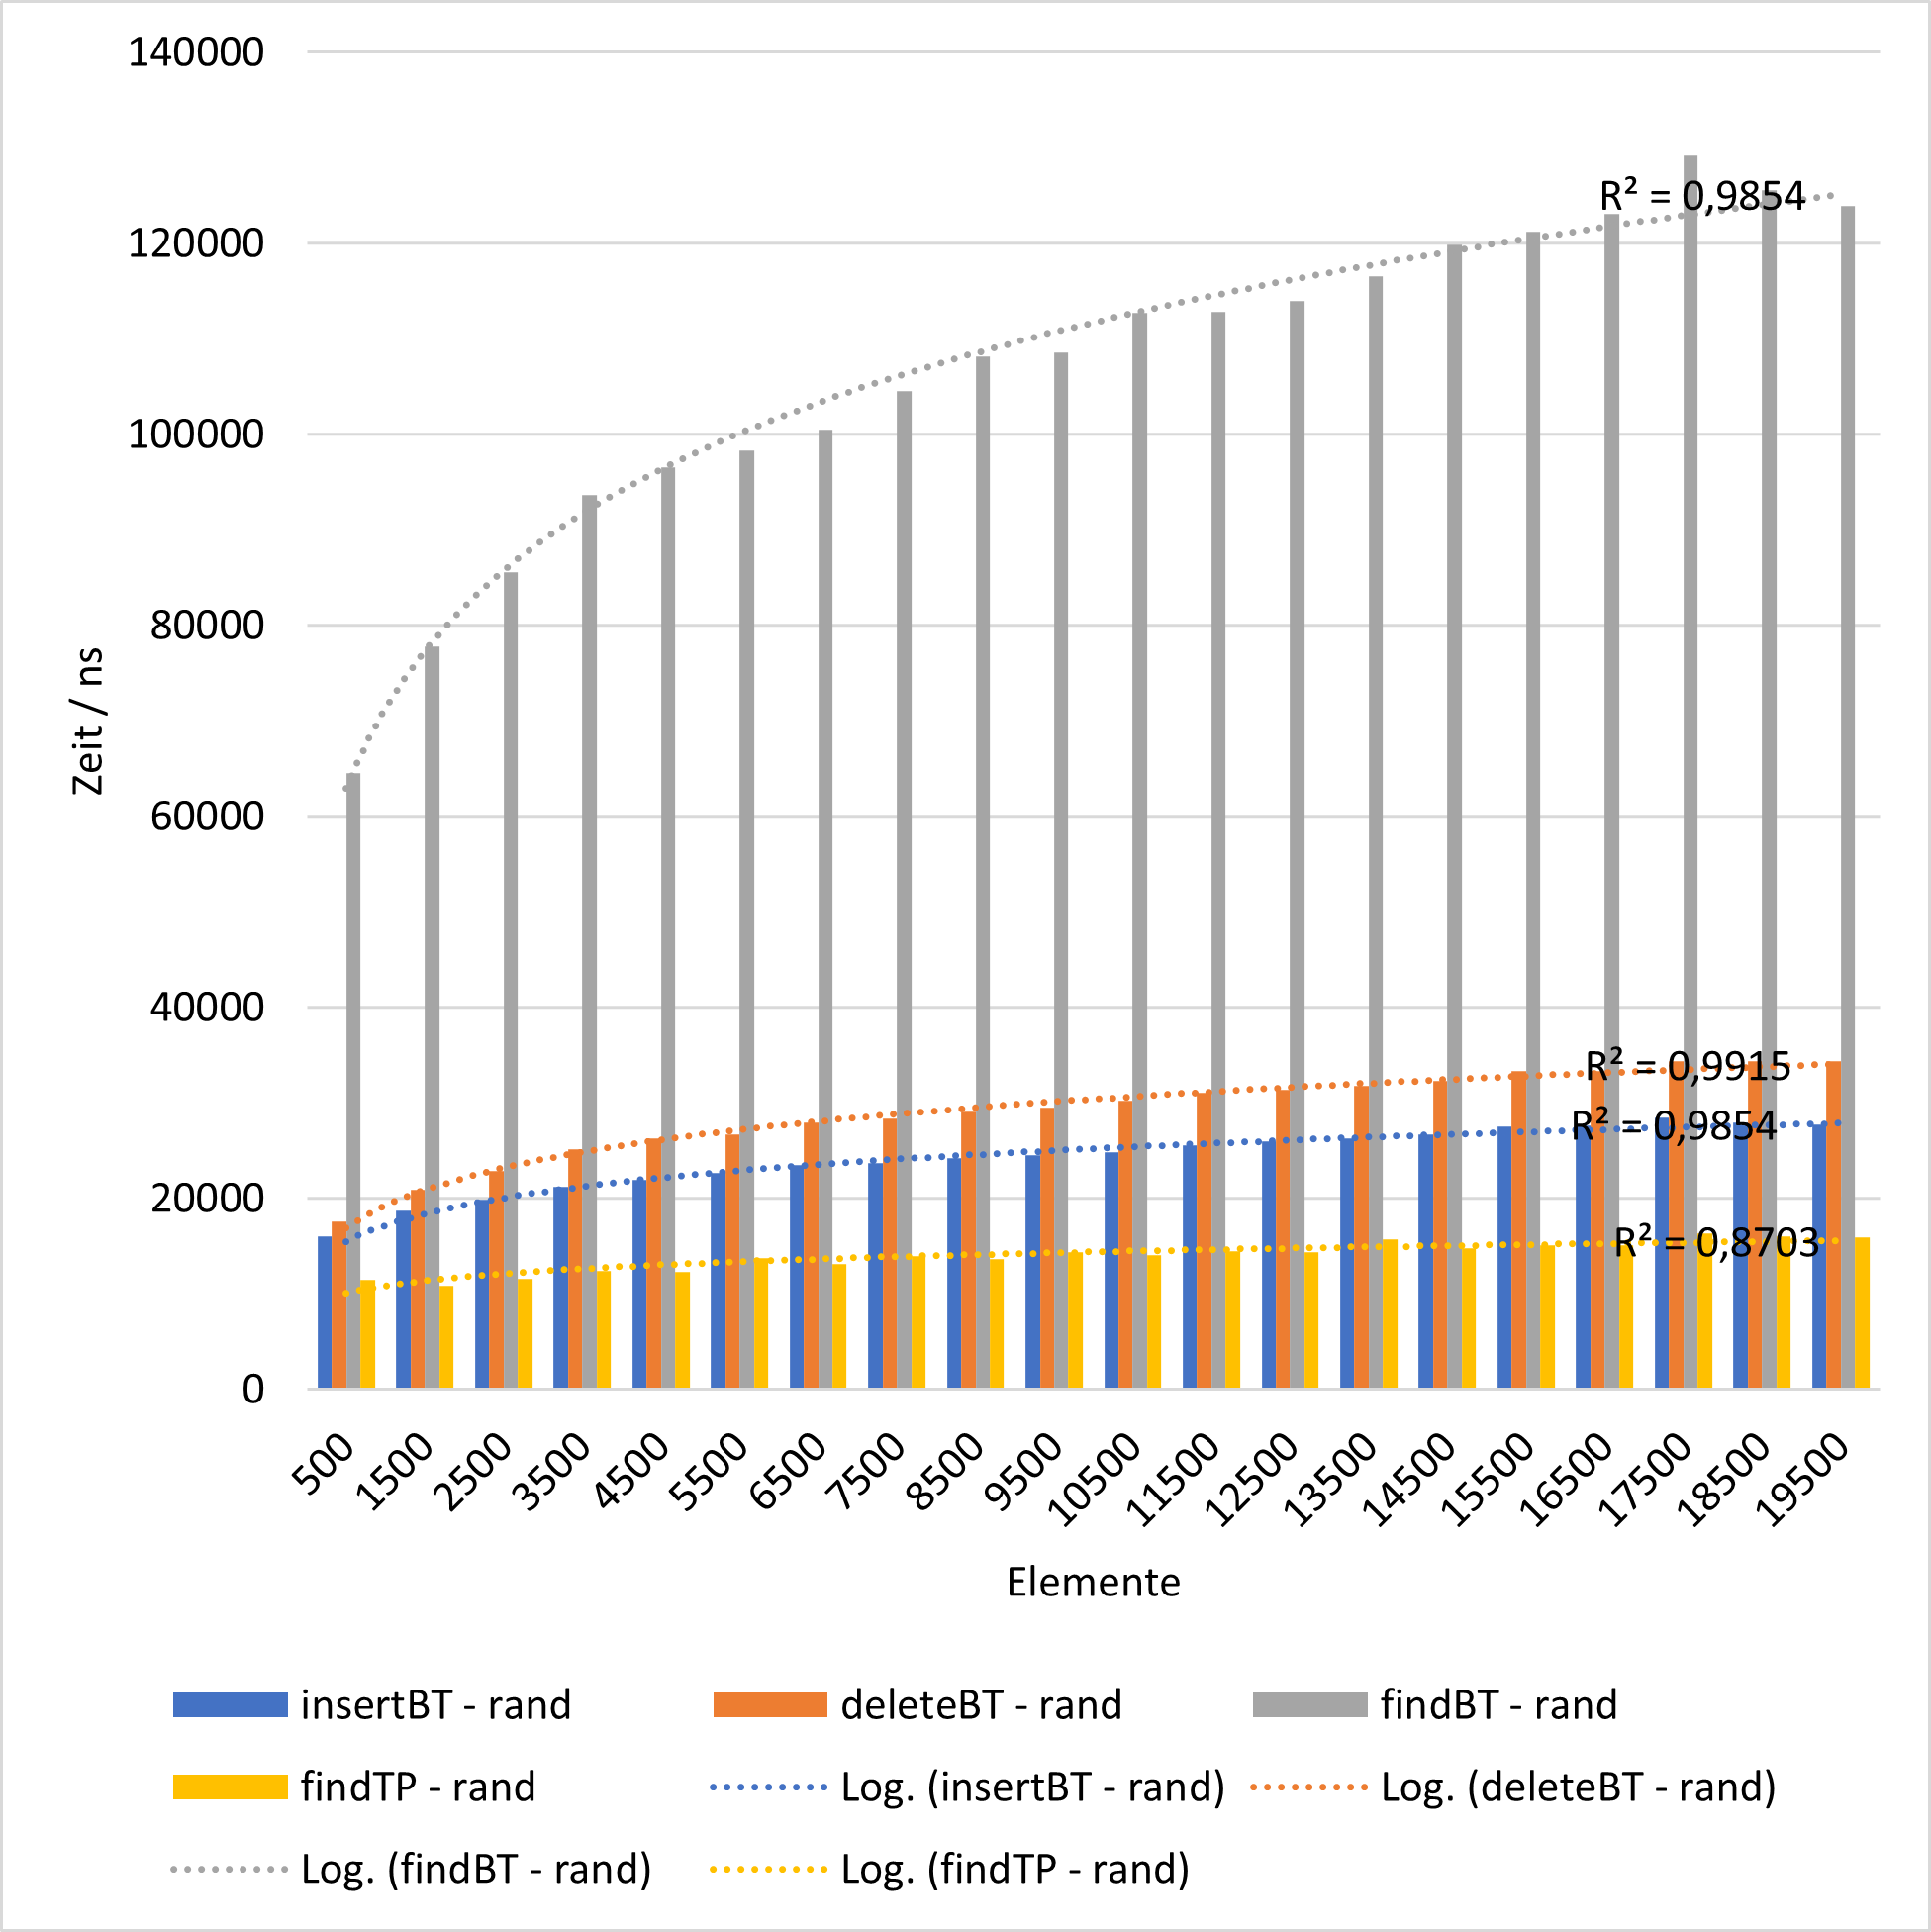
\includegraphics[width = 0.45\textwidth]
        {img/excel/splay_rand_el.png}\label{fig:splay-zeit-rand-el}}
    \caption{Zeitmessungen Splay-Baum}
    \label{fig:splay_zeit}
\end{figure}

\begin{figure}[hbt]
    \centering
    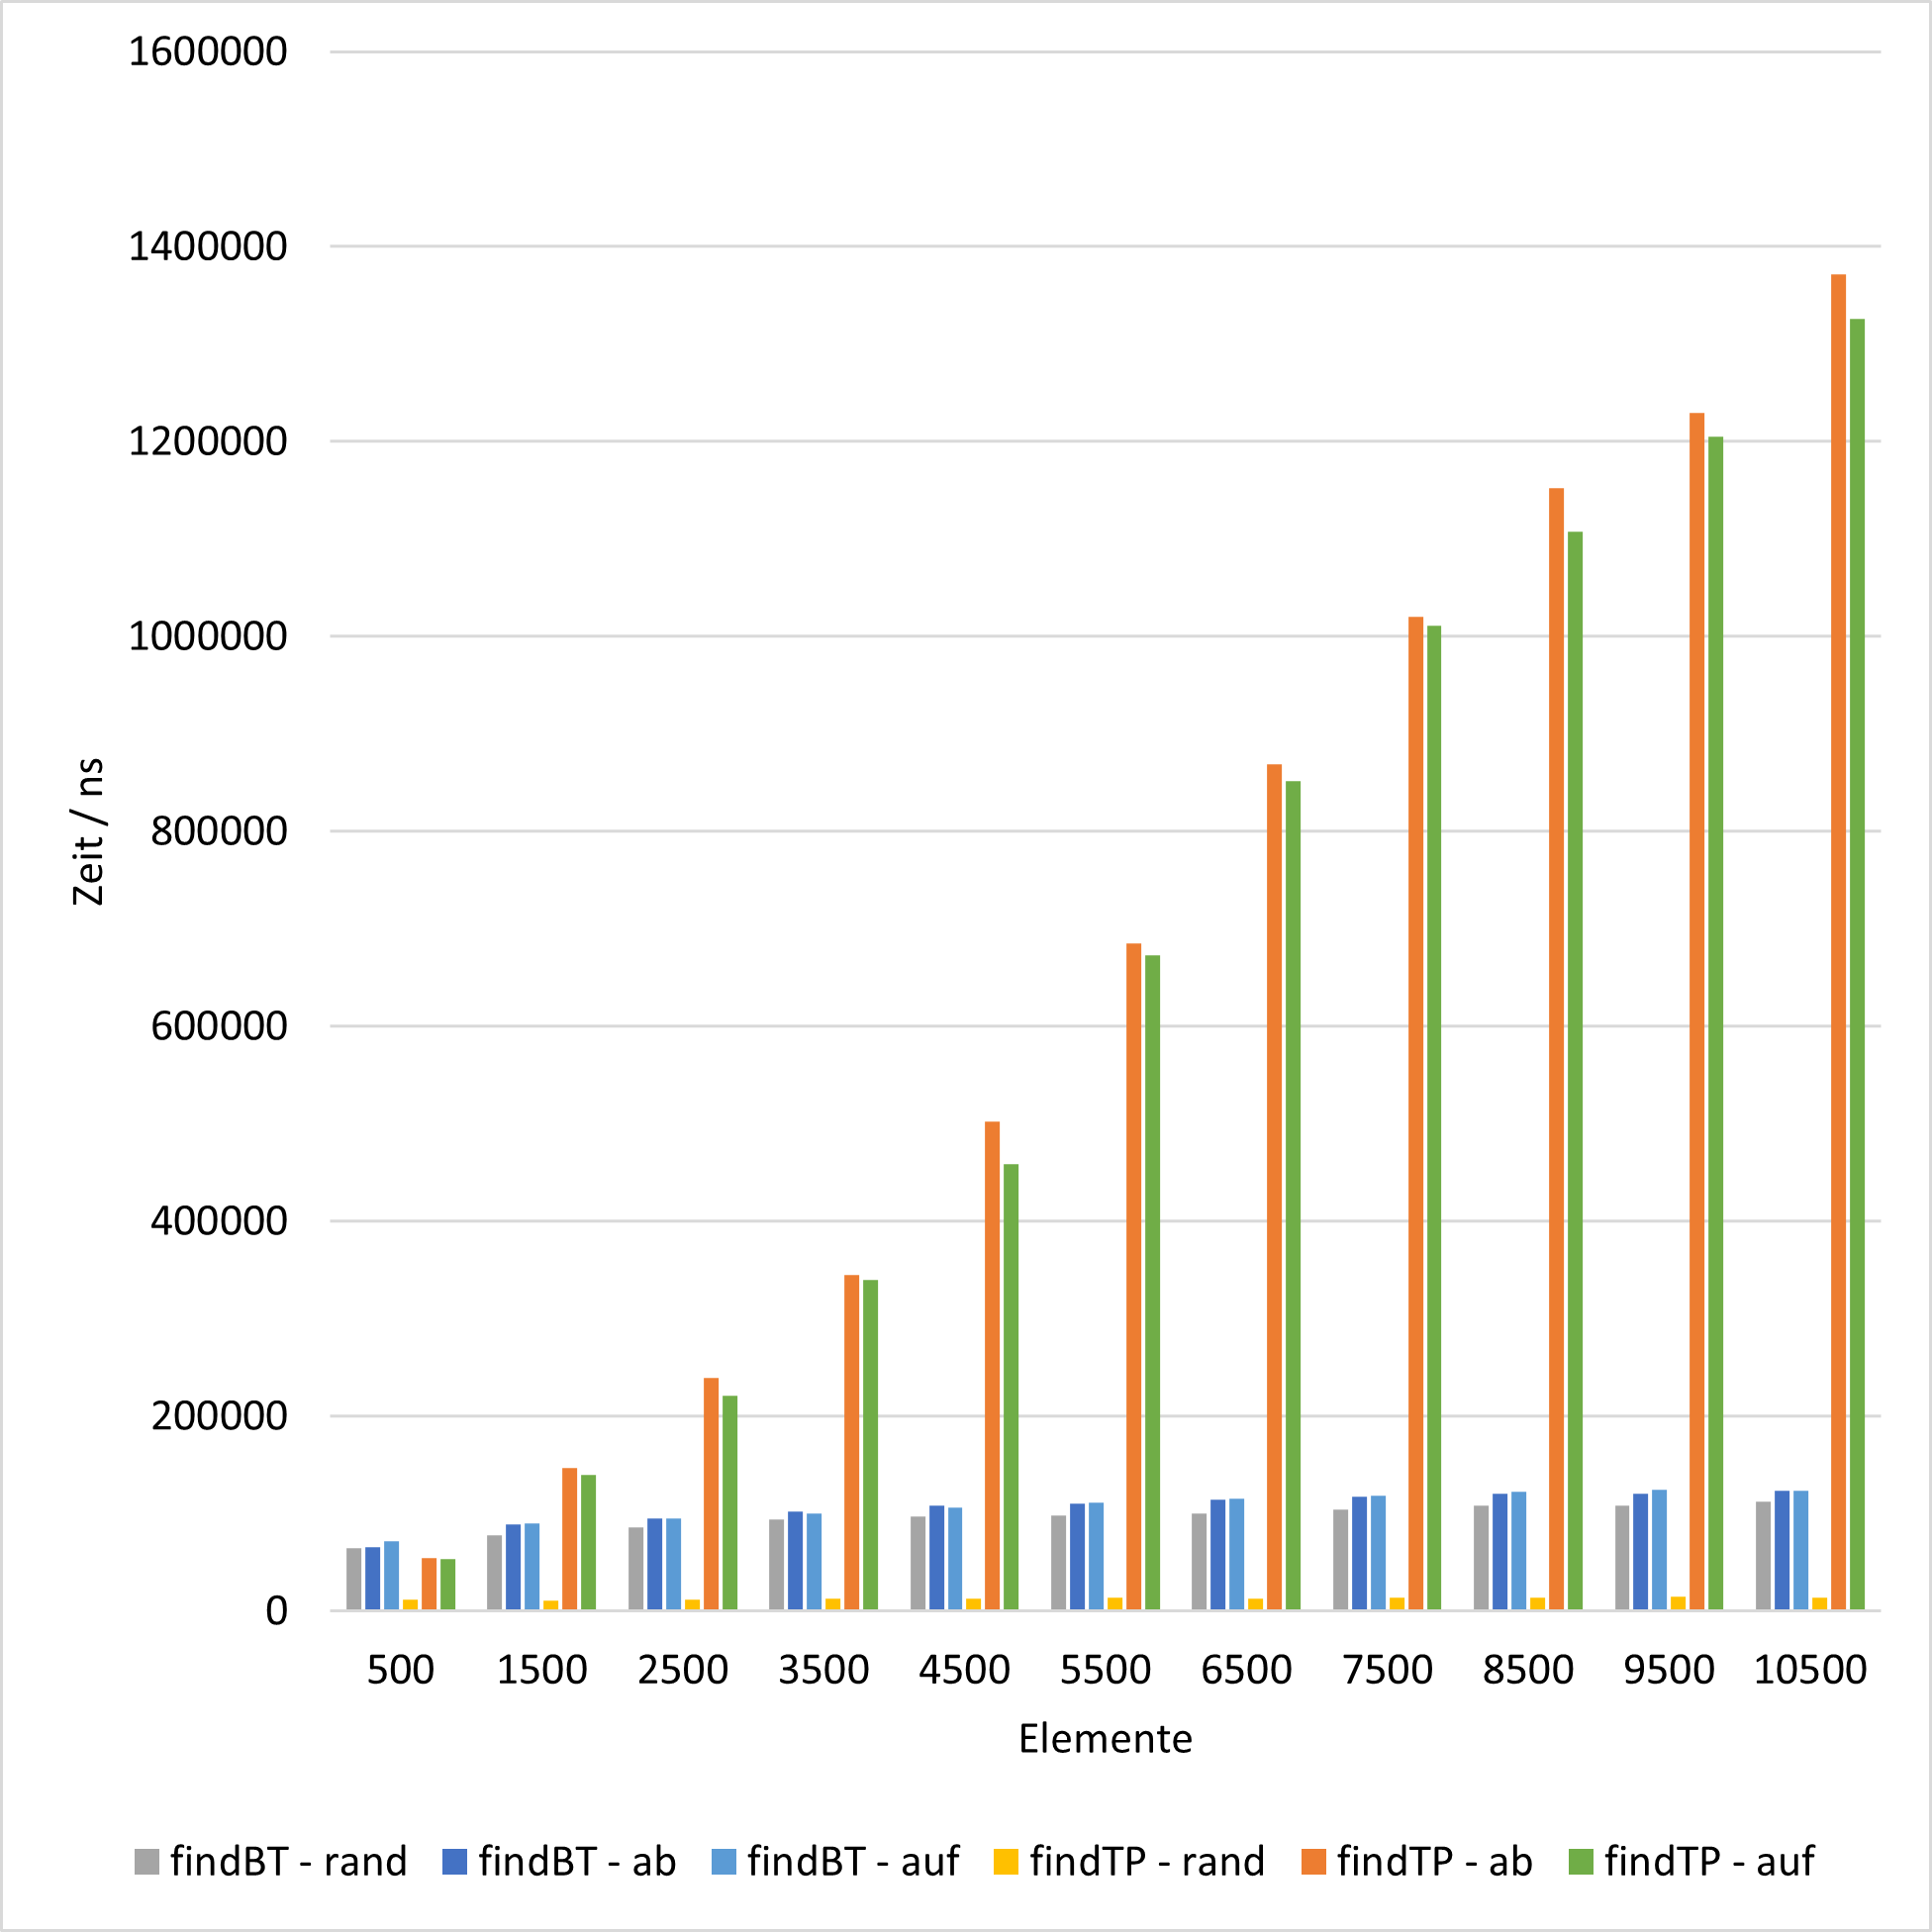
\includegraphics[width=0.45\textwidth]{img/excel/splay_tp_vs_bt.png}
    \caption{Pro Element - FindTP vs. FindBT}
    \label{fig:splay-bt-vs-tp}
\end{figure}


\FloatBarrier
\subsection{Vergleich}